%% ============================================================
%%  main.tex
%%  Longitudinal Analysis of HPC Utilization at a Research University:
%%  Trends, Insights, and Data-Driven Interventions for
%%  Optimized Resource Allocation
%%
%%  Compile with:  pdflatex main.tex  (twice for cross-refs)
%%                 bibtex  main
%%                 pdflatex main.tex
%%                 pdflatex main.tex
%%
%%  Or on Overleaf: set compiler to pdfLaTeX, bibliography tool bibtex.
%% ============================================================

\documentclass[11pt,letterpaper]{article}

%% ---- packages -------------------------------------------------------
\usepackage[margin=1in]{geometry}
\usepackage{amsmath,amssymb}
\usepackage{graphicx}
\usepackage{booktabs}           % professional table rules
\usepackage{tabularx}           % stretchy table columns
\usepackage{array}              % extra column formats
\usepackage{multirow}
\usepackage{xcolor}
\usepackage{hyperref}
\usepackage{url}
\usepackage{microtype}          % better text spacing
\usepackage{setspace}
\usepackage[numbers,sort&compress]{natbib}
\usepackage{caption}
\usepackage{subcaption}
\usepackage{float}
\usepackage{parskip}            % paragraph spacing instead of indent
\usepackage{enumitem}
\usepackage{fancyhdr}
\usepackage{abstract}

%% ---- hyperref setup -------------------------------------------------
\hypersetup{
  colorlinks = true,
  linkcolor  = blue!70!black,
  citecolor  = green!50!black,
  urlcolor   = blue!70!black,
  pdftitle   = {Longitudinal Analysis of HPC Utilization at a Research University},
  pdfauthor  = {GMU Office of Research Computing},
}

%% ---- custom commands ------------------------------------------------
\newcommand{\hopper}{\textsc{Hopper}}
\newcommand{\slurm}{\textsc{Slurm}}
\newcommand{\orc}{ORC}
\newcommand{\gmu}{GMU}
\newcolumntype{R}[1]{>{\raggedleft\arraybackslash}p{#1}}
\newcolumntype{L}[1]{>{\raggedright\arraybackslash}p{#1}}

%% ---- caption style --------------------------------------------------
\captionsetup{
  font       = small,
  labelfont  = bf,
  format     = plain,
  justification = justified,
  singlelinecheck = false,
}

%% ---- header/footer --------------------------------------------------
\pagestyle{fancy}
\fancyhf{}
\lhead{\small\textit{Longitudinal Analysis of HPC Utilization}}
\rhead{\small George Mason University ORC}
\cfoot{\thepage}
\renewcommand{\headrulewidth}{0.4pt}

%% ====================================================================
\begin{document}

%% ---- title block ----------------------------------------------------
\begin{titlepage}
  \centering
  \vspace*{2cm}

  {\LARGE\bfseries Longitudinal Analysis of HPC Utilization\\[0.4em]
   at a Research University: Trends, Insights,\\[0.4em]
   and Data-Driven Interventions for\\[0.4em]
   Optimized Resource Allocation\par}

  \vspace{1.8cm}

  {\large [Author Names]\\[0.3em]
  \textit{Office of Research Computing}\\[0.2em]
  \textit{George Mason University, Fairfax, VA 22030, USA}\\[0.3em]
  \texttt{[contact email]}\par}

  \vspace{1.5cm}

  {\large \today\par}

  \vspace{2cm}

  \begin{abstract}
    \noindent
    The growing adoption of high-performance computing (HPC) resources across
    diverse research disciplines has created an urgent need for data-informed
    approaches to resource allocation and support deployment.  This paper presents
    a longitudinal analysis of utilization patterns on \hopper, the primary HPC
    cluster at George Mason University (\gmu), spanning three academic periods:
    AY~2023--2024, the full calendar year 2025, and the Fall~2025--Spring~2026
    academic semester window.  Drawing on \slurm{} job scheduler records comprising
    over 7.4~million job submissions, we characterize usage trends across compute
    resource types, institutional colleges, academic departments, user cohorts,
    and instructional accounts.  Our analysis reveals three structural shifts:
    (1)~a rapid acceleration of GPU workloads, with daily GPU job counts
    quadrupling between early 2025 and Spring 2026 and GPU-hour consumption
    becoming highly concentrated among a small number of power users;
    (2)~a near-tripling of College of Science (COS) utilization accompanied by
    the emergence of GPU adoption in natural science disciplines; and (3)~the rise
    of the IST department as the single largest job submitter by volume, exhibiting
    a fundamentally different usage profile from other major consumers.  We further
    identify bimodal CPU request distributions indicating systematic
    under-utilisation of shared-memory parallelism and recurring semester-correlated
    queue congestion events reaching average wait times of 4.3~hours.  Based on
    these findings we propose evidence-based interventions spanning personnel
    specialisation, queue policy design, infrastructure planning, and targeted
    outreach.
  \end{abstract}

  \vspace{0.6cm}
  \noindent\textbf{Keywords:} high-performance computing; HPC utilization;
  resource allocation; GPU computing; Slurm; research computing; academic HPC

\end{titlepage}

%% ====================================================================
\setcounter{page}{1}

%% ====================================================================
\section{Introduction}
\label{sec:intro}

High-performance computing has become an essential instrument across the full
breadth of academic research, from the traditionally computation-intensive fields
of physics and engineering to disciplines such as the life sciences, social
science, and the humanities, where computational methods have only recently
become mainstream~\citep{smith2022,nsf2007}.  Institutional HPC centres must
therefore serve an increasingly heterogeneous user population while managing
constrained hardware and personnel resources.  The challenge is not simply
providing sufficient compute capacity; it is deploying that capacity---and the
human expertise needed to use it productively---in ways calibrated to actual
user needs and behaviour.

Most analyses of HPC usage address this challenge from the perspective of aggregate
throughput: total CPU-hours consumed, overall system utilisation rates, and job
success ratios.  These measures are valuable for justifying institutional investment
but provide limited guidance for operational decision-making~\citep{cahill2014,vonlaszewski2012}.
A growing body of work has demonstrated that disaggregated analysis---examining
usage by discipline, user role, job type, and temporal pattern---yields actionable
insights invisible in aggregate statistics~\citep{furlani2013,simakov2018}.
Understanding that a particular department submits thousands of very short jobs
while another submits dozens of multi-day parallel simulations has direct
implications for queue configuration, support priority, and training content,
even when the aggregate resource consumption of the two groups is similar.

This paper extends the framework introduced in our earlier work on optimising HPC
resource deployment at \gmu~\citep{orc2022internal} through a systematic
longitudinal analysis of \hopper{} cluster utilisation spanning from the
2023--2024 academic year through Spring~2026.  Three findings motivate the core
contributions.  First, GPU workloads have grown dramatically and now exhibit
levels of concentration---a single user consuming more GPU-hours than the next
six combined over a nine-month window---that raise questions about equitable
access in a shared resource environment.  Second, the College of Science,
historically a secondary user of \hopper{} primarily running CPU-based
simulations, has nearly tripled its utilisation and is beginning to adopt GPU
workflows in atmospheric modelling, structural biology, and chemistry.  Third,
the IST department has become the largest single job submitter in the university
by count while simultaneously having the lowest average per-job resource
consumption, a mismatch that challenges conventional assumptions about who the
``heavy users'' are and what form effective support should take.

The paper proceeds as follows.  Section~\ref{sec:related} reviews related work.
Section~\ref{sec:system} describes the \hopper{} system and data sources.
Section~\ref{sec:method} presents the analytical methodology.
Section~\ref{sec:results} reports the empirical findings.
Section~\ref{sec:discussion} interprets these findings.
Section~\ref{sec:interventions} translates the analysis into specific,
evidence-based interventions.  Section~\ref{sec:conclusion} concludes.

%% ====================================================================
\section{Background and Related Work}
\label{sec:related}

\subsection{HPC Utilisation Analysis}

The systematic analysis of HPC usage statistics has a well-established tradition
in the research computing community.  Early work focused primarily on demonstrating
the productivity impact of HPC investment: \citet{smith2022} showed that
computational researchers produce statistically significantly more research output
than non-computational peers across disciplines.  \citet{furlani2013} developed
the XDMoD framework, which operationalises a broad range of utilisation metrics
enabling systematic analysis at both national XSEDE scale and at individual
institutional centres.  \citet{hammond2011} extended this approach to I/O
performance monitoring.

More recent work has examined utilisation patterns in relation to user support
and training.  \citet{kilpatrick2019} demonstrated that users who receive targeted
consultation from research computing facilitators show measurable improvements in
job efficiency.  A complementary line of research has examined the relationship
between system complexity and user error rates, finding that the barrier of
command-line \slurm{} job submission is a major source of both inefficiency and
support burden~\citep{ragavan2020}.  The deployment of web-based interfaces such
as Open OnDemand has been shown to reduce this barrier and increase effective
cluster utilisation among non-specialist researchers~\citep{hudak2016}.

\subsection{GPU Computing in Academic HPC}

The rapid diffusion of GPU-accelerated workloads into academic HPC environments
has introduced new challenges for resource management.  \citet{netti2019} analysed
GPU utilisation across a large European HPC facility and found that a small
fraction of users---typically 10--15\%---account for 60--80\% of GPU-hours
consumed, a concentration pattern consistent with what we observe at \gmu.
\citet{chard2015} examined the impact of GPU demand growth on queue dynamics,
showing that wait-time inflation during peak periods is disproportionately driven
by large-GPU-count jobs submitted by a small number of users.

\subsection{Instructional HPC Use}

The use of HPC clusters for formal coursework represents a qualitatively distinct
usage pattern from research computing.  Instructional jobs are characterised by
high submission synchronicity, short individual job duration, and strong temporal
correlation with the academic calendar~\citep{sill2020}.  The expansion of data
science and machine learning curricula has accelerated the instructional demand
for GPU resources specifically~\citep{wehner2021}.

\subsection{Resource Allocation Under CaRCC Frameworks}

The Campaign for Research Computing Competencies (CaRCC) has articulated a
structured framework for classifying research computing personnel activities
into four facings: researcher-facing, system-facing, software/data-facing, and
sponsor/stakeholder-facing~\citep{carcc2022}.  Our earlier work~\citep{orc2022internal}
introduced the linkage between utilisation analysis and CaRCC-structured personnel
deployment; the present analysis provides the longitudinal data needed to assess
how the composition of support needs has changed over time.

%% ====================================================================
\section{System Description and Data Sources}
\label{sec:system}

\subsection{The Hopper Cluster}

\hopper{} is the primary HPC cluster operated by the \gmu{} Office of Research
Computing (\orc).  At the time of this analysis, \hopper{} comprises approximately
11,840~CPU cores, a VAST flash-based scratch storage system, and a heterogeneous
GPU partition including NVIDIA A100 (40\,GB and 80\,GB), A40, H100, and B200
class GPUs accessed via MIG and full-device configurations.  Users access \hopper{}
via SSH connections to login nodes or through the \orc{} Open OnDemand (OOD) web
interface~\citep{hudak2016}.  Job scheduling is managed by the \slurm{} Workload
Manager~\citep{yoo2003}.

\subsection{Data Sources and Coverage}

The primary data source is the \slurm{} job accounting database, from which
records were extracted covering three non-overlapping periods:

\begin{itemize}[leftmargin=2em]
  \item \textbf{AY~2023--2024}: July~2023 through June~2024 (12~months,
        baseline period).
  \item \textbf{Full Year~2025}: January~2025 through December~2025
        (12~months, retrospective period).
  \item \textbf{Fall~2025--Spring~2026}: August~2025 through April~2026
        (9~months, current period).
\end{itemize}

For each completed job the extracted record includes: user identifier
(anonymised), account identifier, submit time, start time, end time, requested
CPUs (NCPUS), requested GPUs (NGPUS), requested nodes (NNODES), requested
memory (GB), consumed CPU-hours (CPUHRS), consumed GPU-hours (GPUHRS), and job
exit state.  Instructional accounts are identifiable by a naming convention
encoding the course prefix, number, and semester code (e.g., \texttt{cs678fl25}
for CS~678, Fall~2025).

%% ====================================================================
\section{Methodology}
\label{sec:method}

\subsection{Metrics}

We report the following utilisation metrics, computed per job and aggregated over
monthly, semester, or annual time windows:

\begin{itemize}[leftmargin=2em]
  \item \textbf{Total jobs}: count of completed records, disaggregated by CPU
        vs.\ GPU (jobs with NGPUS\,$>$\,0).
  \item \textbf{CPU-hours (CPUHRS)}: product of allocated CPUs and elapsed wall
        time.
  \item \textbf{GPU-hours (GPUHRS)}: product of allocated GPUs and elapsed wall
        time.
  \item \textbf{Average memory requested}: mean allocation in GB per job.
  \item \textbf{Average wall time} and \textbf{average wait time}: mean elapsed
        and queueing durations in hours.
  \item \textbf{Active unique users}: distinct user identifiers submitting at
        least one job in a given time window.
\end{itemize}

\subsection{Classification and Longitudinal Comparison}

Jobs are classified as \emph{CPU jobs} if NGPUS\,=\,0 and \emph{GPU jobs} if
NGPUS\,$>$\,0.  Institutional affiliations are classified at college and
department levels.  Instructional accounts are treated as a distinct stratum.
Longitudinal comparisons normalise to a per-month basis where windows of
different length are compared.

%% ====================================================================
\section{Results}
\label{sec:results}

\subsection{Overall Utilisation Trends}

Total job volume increased substantially across the three analysis periods.
The Full Year~2025 retrospective recorded \textbf{2,283,321} total job
submissions (CPU:~2,159,248; GPU:~124,073).  The Fall~2025--Spring~2026
nine-month window recorded \textbf{2,905,604} total submissions
(CPU:~2,777,817; GPU:~127,787).  That a nine-month period exceeds the full
2025 yearly total confirms a strong upward volume trend.
Figure~\ref{fig:annual_volume} shows the aggregate statistics across all three
periods.

\begin{figure}[H]
  \centering
  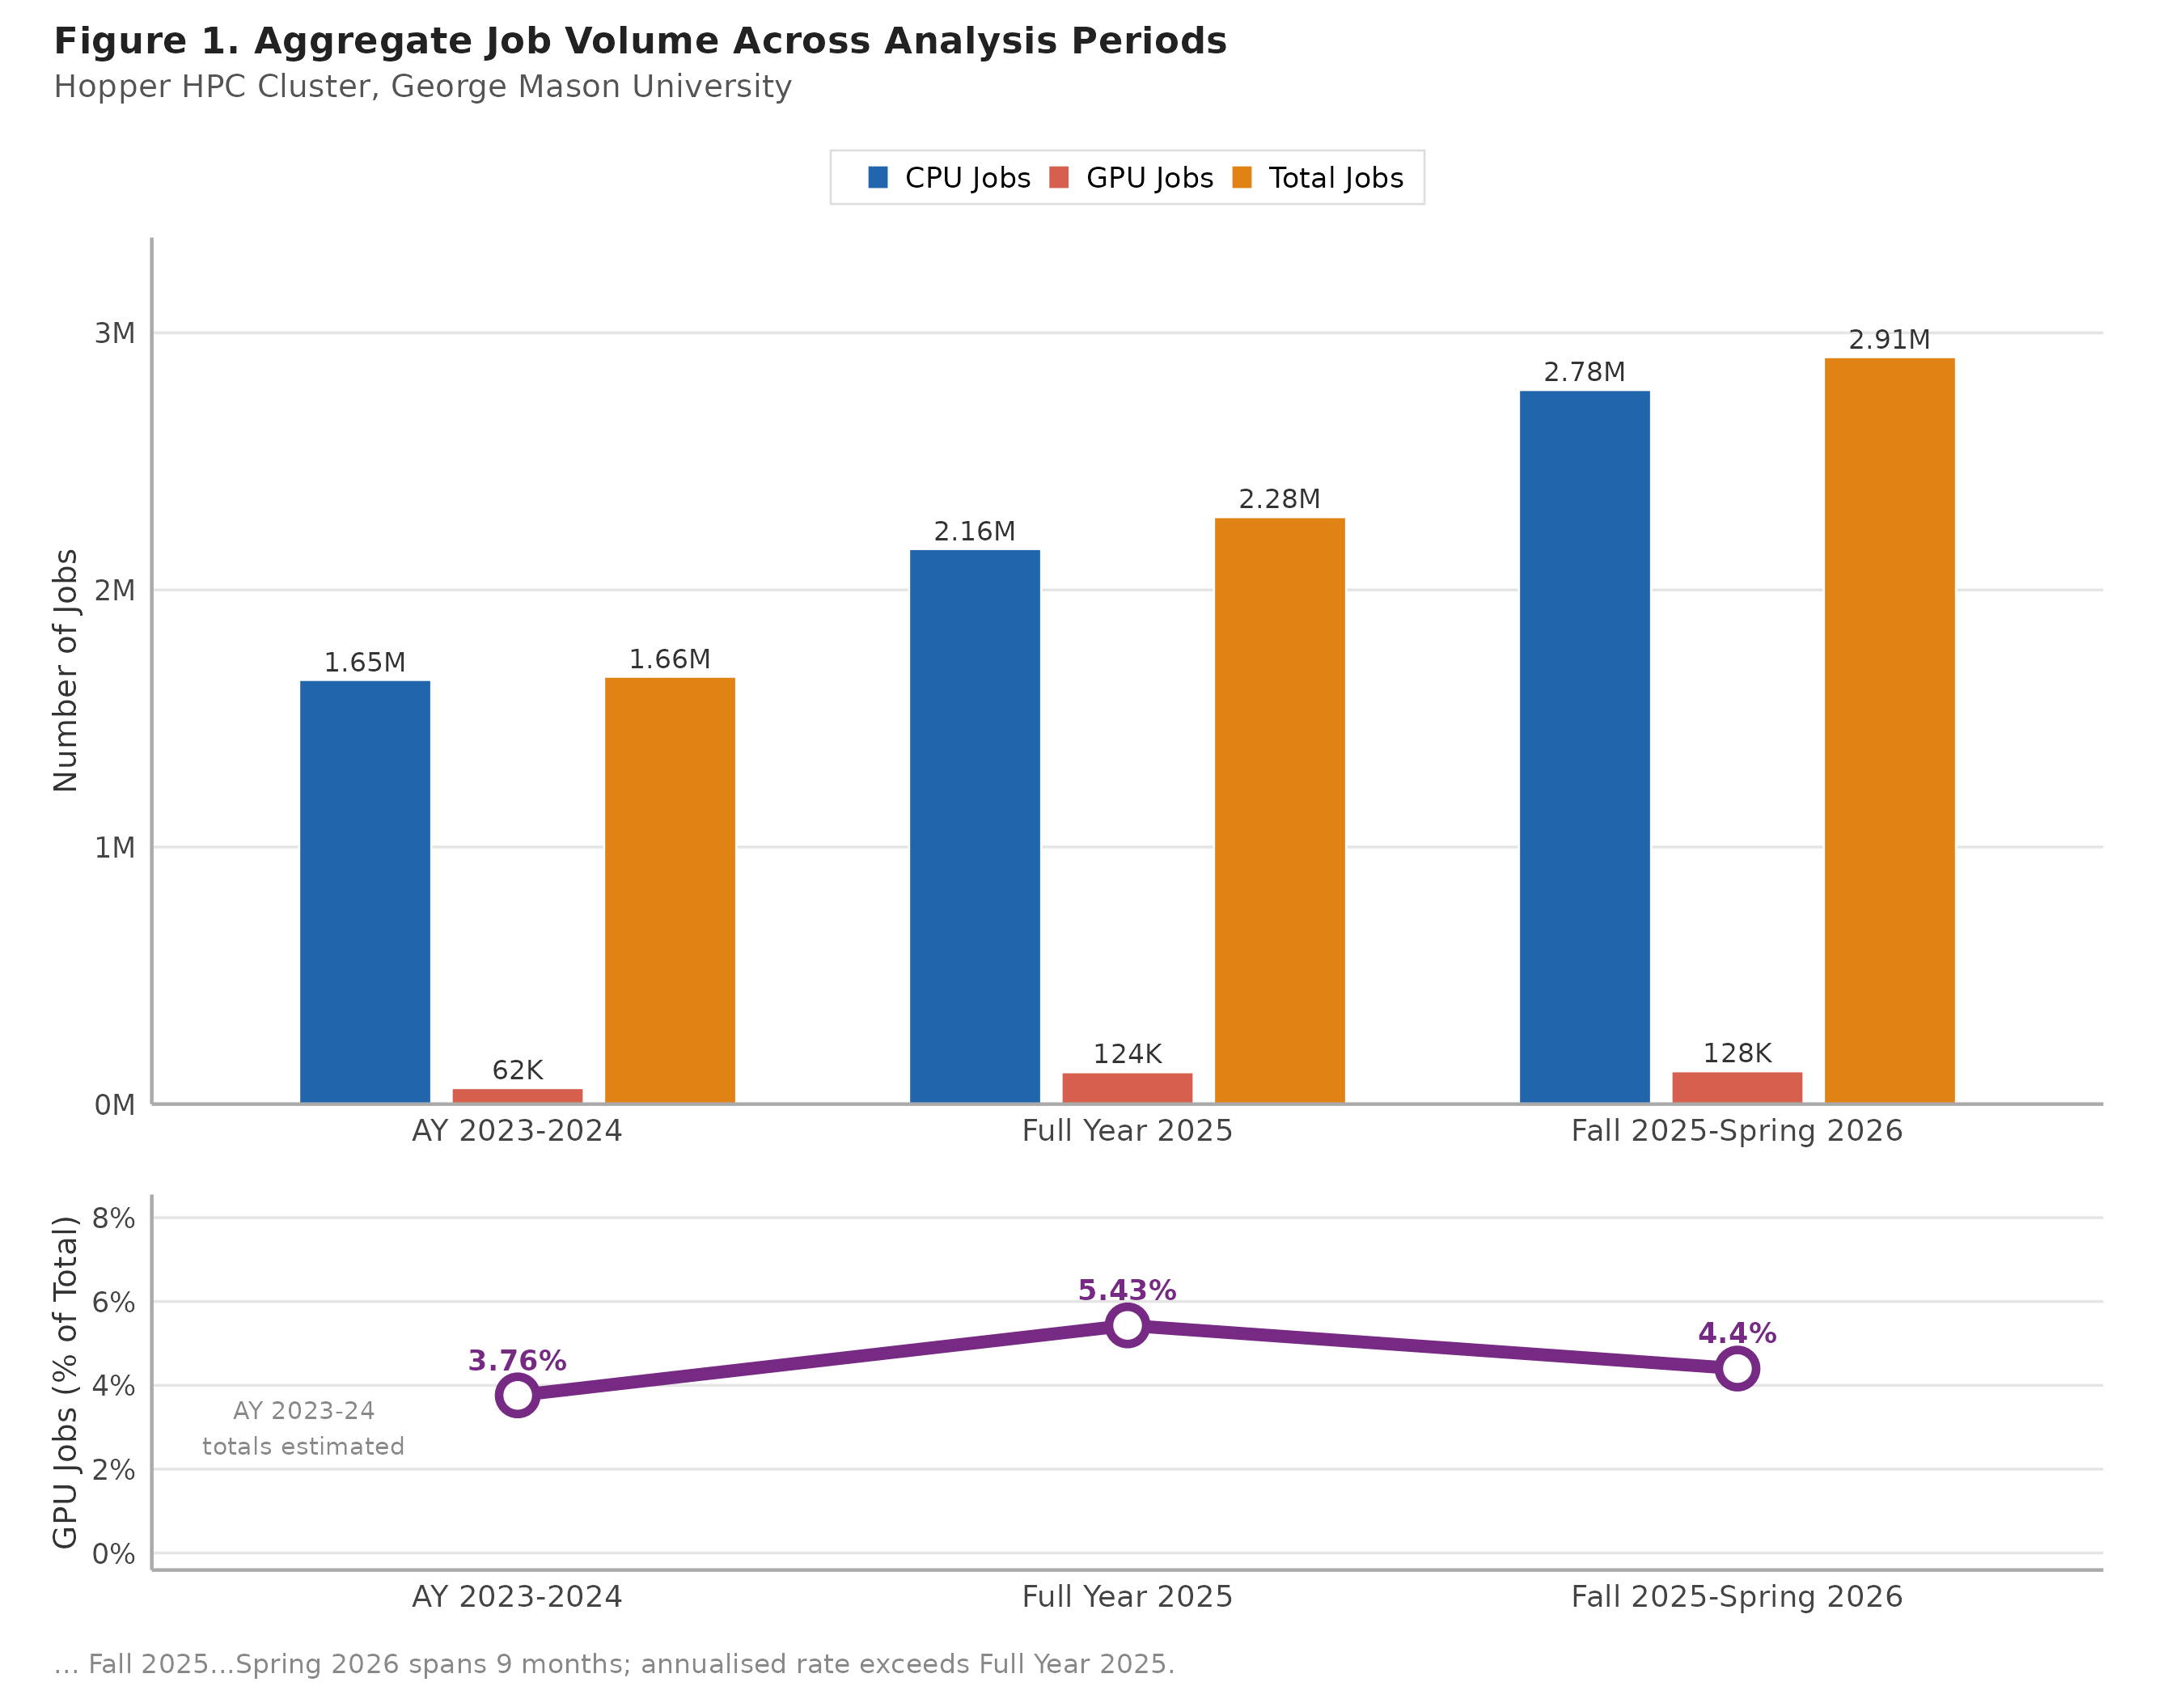
\includegraphics[width=\textwidth]{figures/fig1_annual_volume.png}
  \caption{Aggregate job volume across all three analysis periods.  CPU~jobs,
    GPU~jobs, and totals are shown as grouped bars (left axis); the GPU
    percentage of total submissions is plotted as a connected line series
    (right axis, purple).  AY~2023--2024 totals are estimated from the
    reported range midpoint.  The Fall~2025--Spring~2026 bar spans only nine
    months; its annualised rate exceeds the Full Year~2025 total.}
  \label{fig:annual_volume}
\end{figure}

Table~\ref{tab:annual} summarises the aggregate statistics.

\begin{table}[H]
  \centering
  \caption{Aggregate utilisation statistics across analysis periods.}
  \label{tab:annual}
  \small
  \begin{tabularx}{\textwidth}{L{3.8cm} R{1.4cm} R{2.0cm} R{1.8cm} R{1.8cm} R{1.6cm}}
    \toprule
    \textbf{Period} & \textbf{Months} & \textbf{CPU Jobs} &
    \textbf{GPU Jobs} & \textbf{Total Jobs} & \textbf{GPU \%} \\
    \midrule
    AY~2023--2024     & 12 & $\sim$1.65M* & $\sim$62.5K* & $\sim$1.66M* & $\sim$3.8\% \\
    Full Year 2025    & 12 & 2,159,248    & 124,073      & 2,283,321    & 5.4\%       \\
    Fall 2025--Spr.\ 2026 & 9  & 2,777,817 & 127,787    & 2,905,604    & 4.4\%       \\
    \bottomrule
  \end{tabularx}
  \smallskip\par
  \raggedright\footnotesize * Estimated from range midpoint; exact aggregate not
  extracted in original analysis.
\end{table}

Monthly job submission patterns reveal pronounced seasonality.  In Full Year~2025,
September (367,874 CPU jobs), October (323,931), and February (312,983) were the
highest-volume months.  July (58,043 CPU jobs) was the lowest, confirming a summer
trough consistent with patterns at comparable academic facilities~\citep{sill2020}.
Average daily unique active users peaked at 617 on Tuesdays in the 2025 data.
Weekend averages remained substantial (506--514 per day in 2025;
320--323 per day in Fall~2025--Spring~2026), indicating a large self-directed user
population.

\subsection{College-Level Utilisation}

Figure~\ref{fig:college} presents the distribution of job submissions by
institutional college in the Fall~2025--Spring~2026 period, and
Table~\ref{tab:college} provides the numerical breakdown.

\begin{figure}[H]
  \centering
  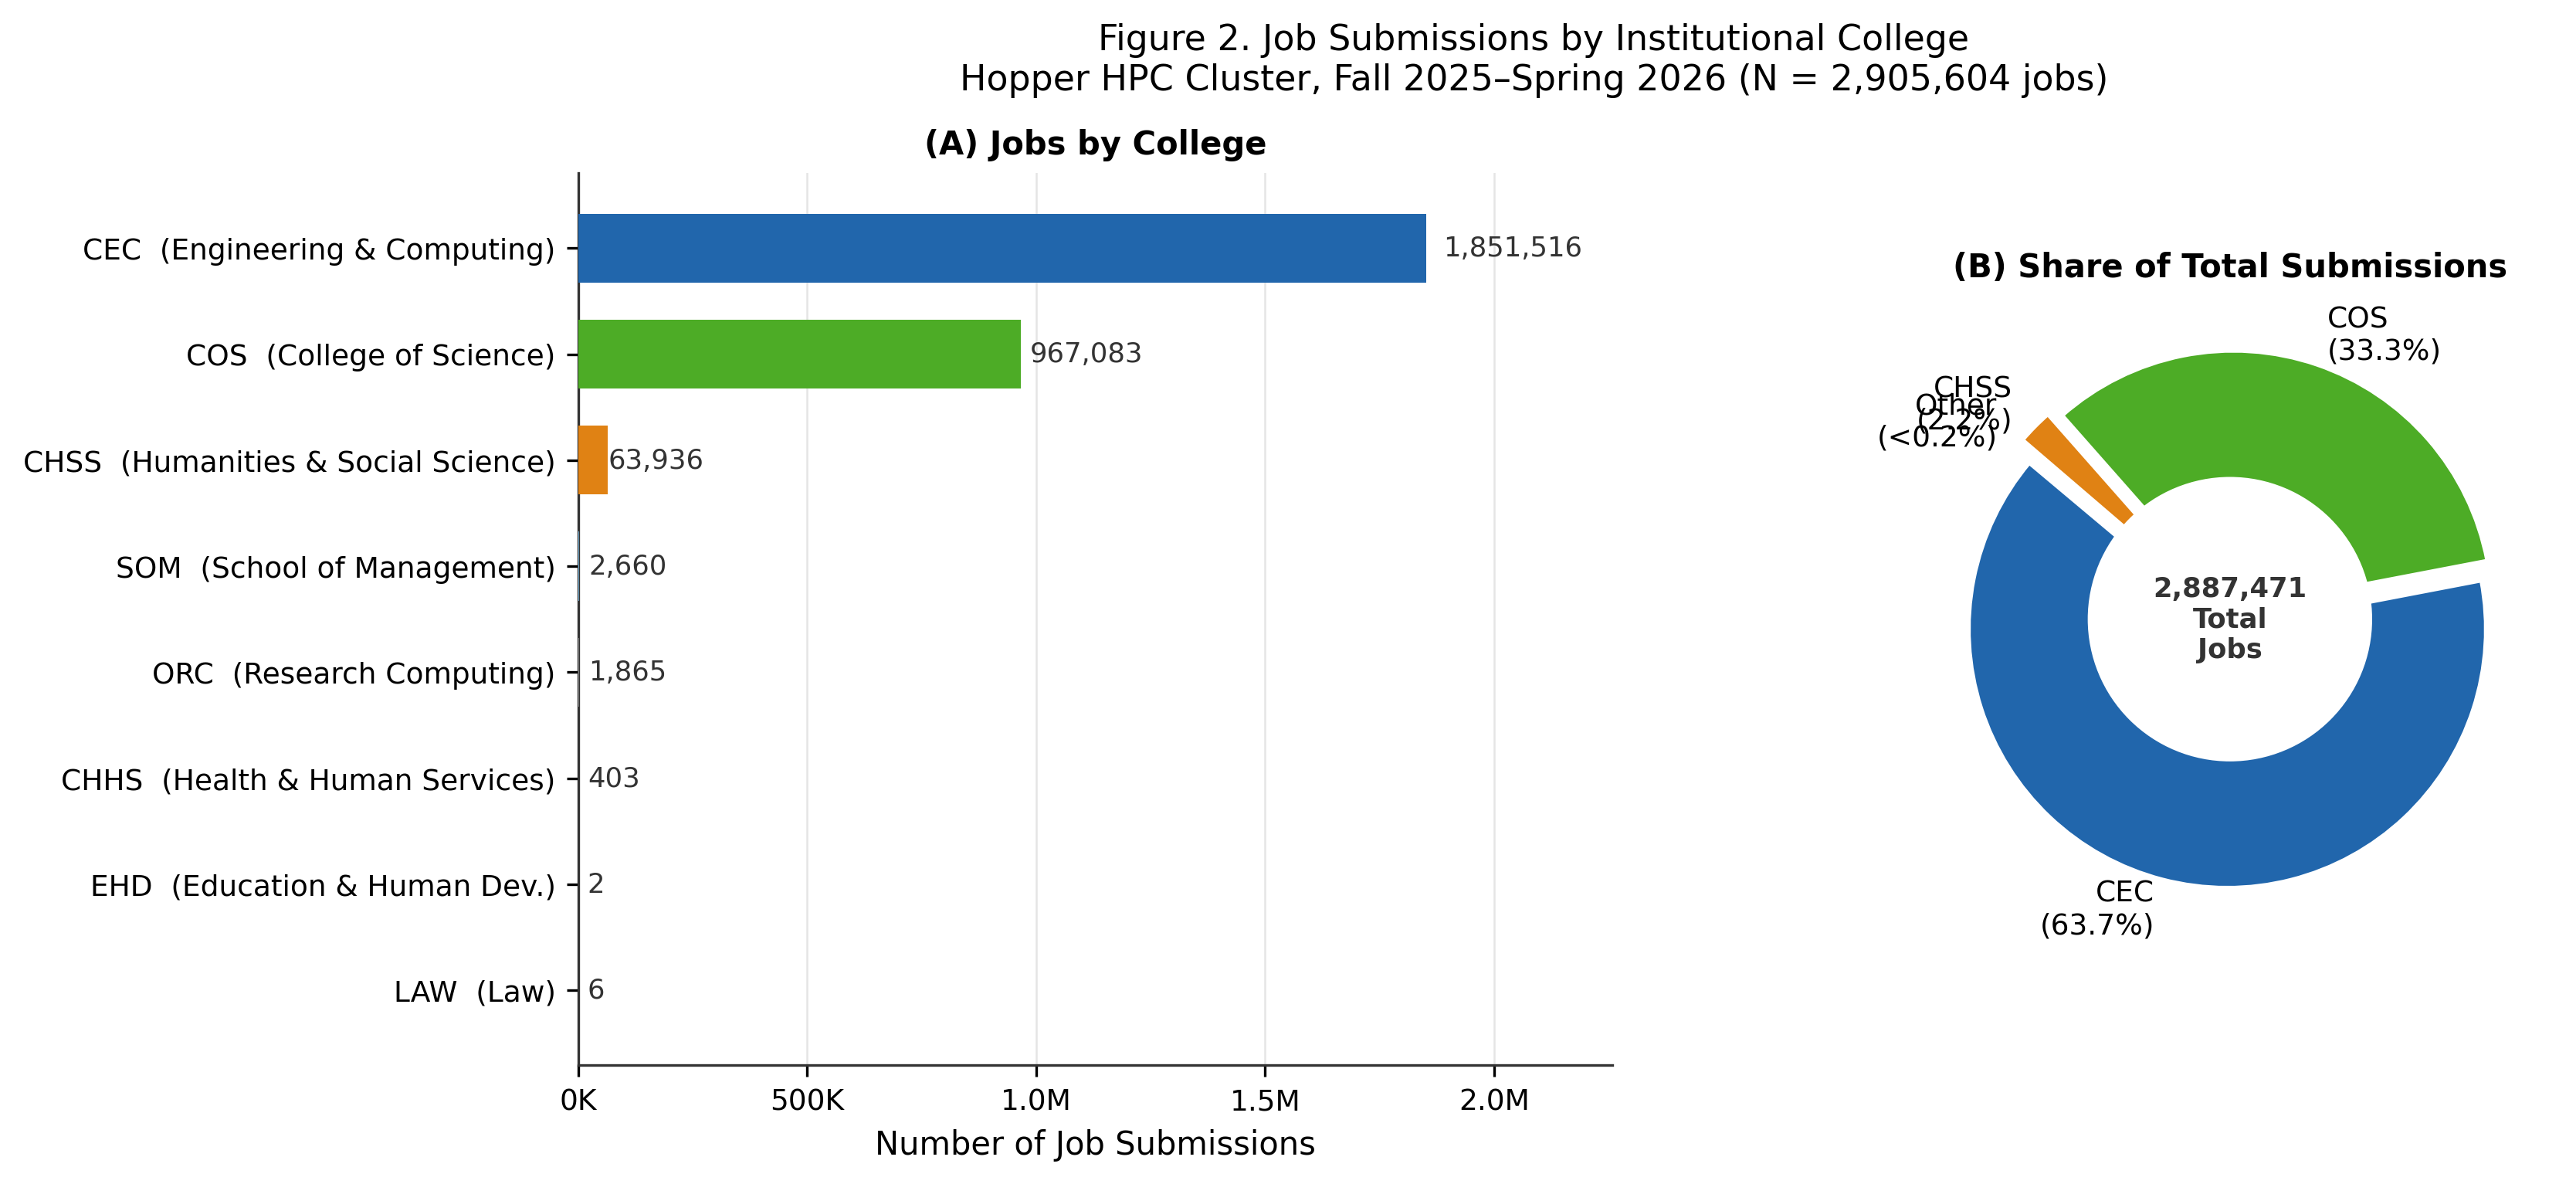
\includegraphics[width=\textwidth]{figures/fig2_college_jobs.png}
  \caption{Job submissions by institutional college, Fall~2025--Spring~2026
    (N\,=\,2,905,604).  Panel~(A): horizontal bar chart of absolute job counts.
    Panel~(B): donut chart showing the share of total submissions; small colleges
    (SOM, ORC, CHHS, EHD, LAW) are aggregated as ``Other'' ($<$0.2\,\%).}
  \label{fig:college}
\end{figure}

\begin{table}[H]
  \centering
  \caption{Job submissions by institutional college, Fall~2025--Spring~2026.}
  \label{tab:college}
  \small
  \begin{tabularx}{0.72\textwidth}{l R{2.8cm} R{2.2cm}}
    \toprule
    \textbf{College} & \textbf{Jobs} & \textbf{Share (\%)} \\
    \midrule
    CEC (Engineering \& Computing)      & 1,851,516 & 63.7 \\
    COS (College of Science)            & 967,083   & 33.3 \\
    CHSS (Humanities \& Social Science) & 63,936    & 2.2  \\
    SOM (School of Management)          & 2,660     & 0.1  \\
    Other (ORC, CHHS, EHD, LAW)        & $<$2,300  & $<$0.1 \\
    \bottomrule
  \end{tabularx}
\end{table}

The COS figure represents a qualitative shift: in Full Year~2025, COS submitted
342,096 CPU jobs over 12~months.  The subsequent nine-month window records
967,083~jobs---a 2.8-fold increase in annualised rate---indicating that COS has
undergone a phase transition from a secondary to a co-primary user of \hopper{}
resources.

\subsection{Department-Level Analysis: CEC}
\label{sec:cec}

Figure~\ref{fig:dept} presents department-level resource profiles.  Within CEC,
Table~\ref{tab:cec_cpu} summarises CPU job statistics.

\begin{figure}[H]
  \centering
  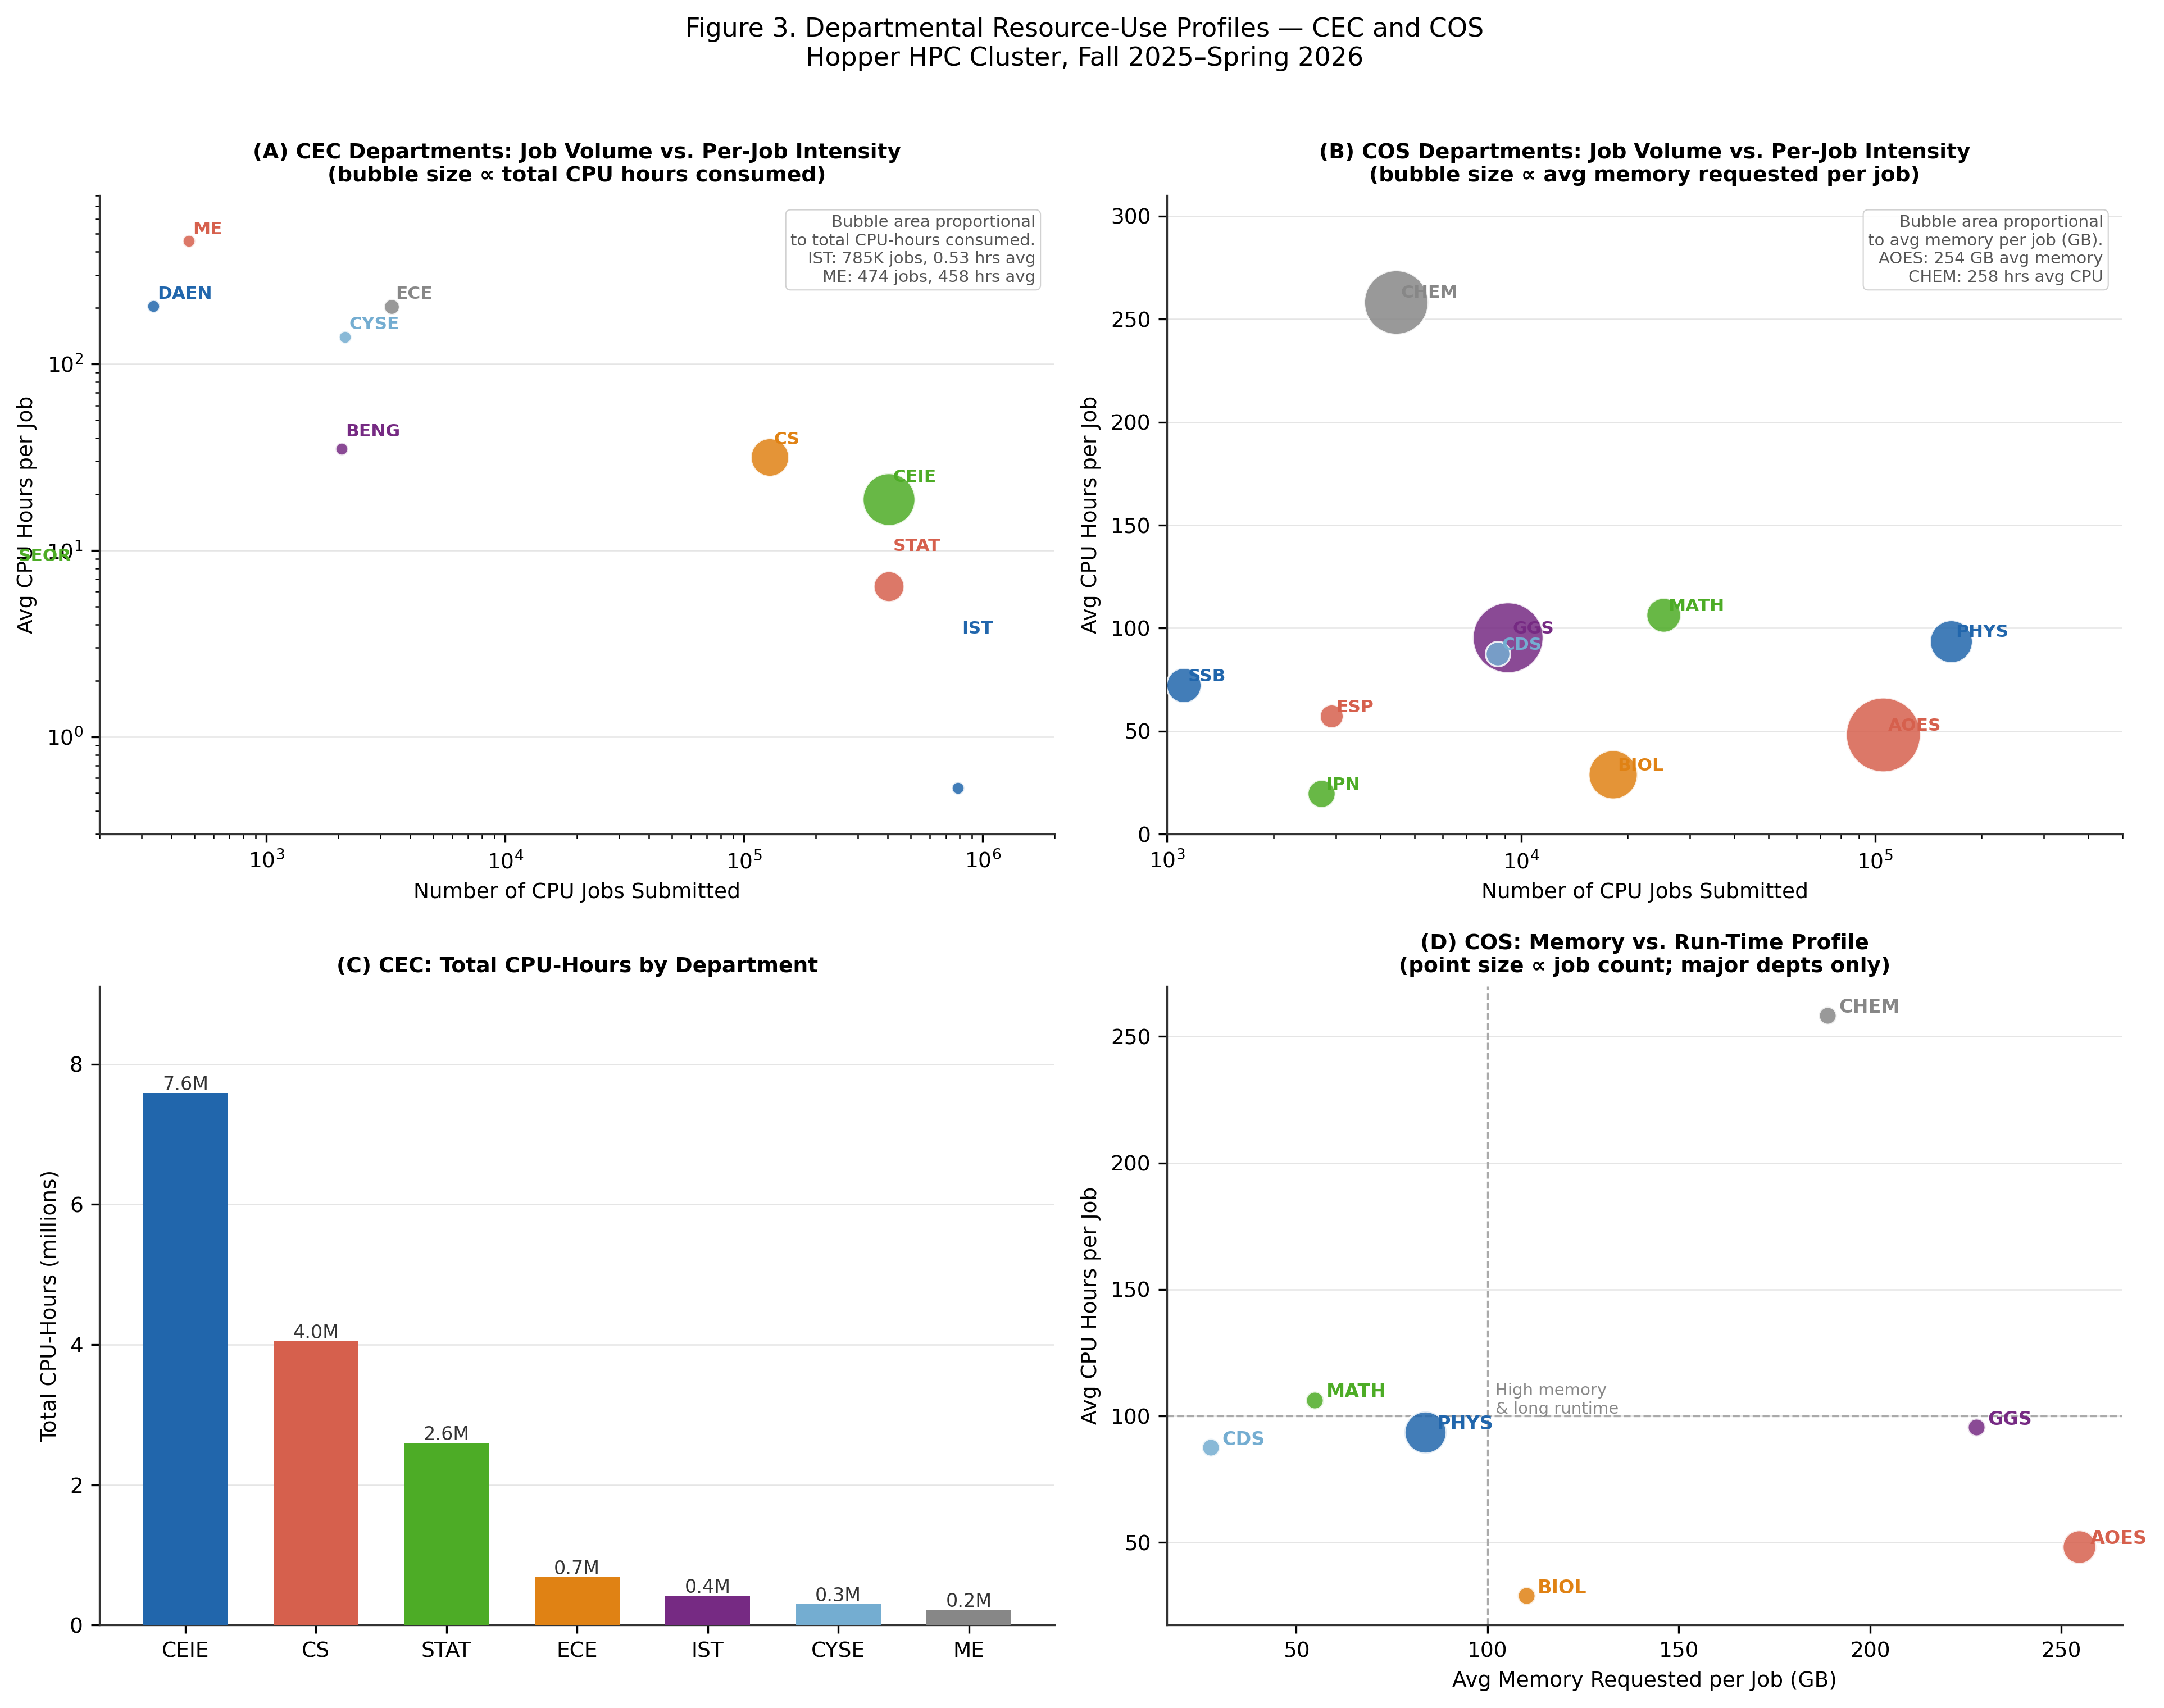
\includegraphics[width=\textwidth]{figures/fig3_department_comparison.png}
  \caption{Departmental resource-use profiles for CEC (Panels~A, C) and COS
    (Panels~B, D).  Bubble charts~(A, B) plot job count vs.\ average CPU-hours
    per job on logarithmic axes; bubble area is proportional to total CPU-hours
    (A) or average memory per job (B).  Bar charts~(C, D) compare total
    CPU-hours across departments and, for COS, plot average memory against
    average run time.}
  \label{fig:dept}
\end{figure}

\begin{table}[H]
  \centering
  \caption{CEC CPU job statistics by department, Fall~2025--Spring~2026.}
  \label{tab:cec_cpu}
  \small
  \begin{tabularx}{\textwidth}{l R{1.8cm} R{2.4cm} R{2.4cm} R{2.2cm}}
    \toprule
    \textbf{Department} & \textbf{CPU Jobs} & \textbf{Total CPU Hrs} &
    \textbf{Avg CPU Hrs/Job} & \textbf{Avg Mem (GB)} \\
    \midrule
    IST (Info.\ Sciences \& Tech.)     & 785,603 & 417,913     & 0.53   & 4.10  \\
    STAT (Statistics)                  & 404,830 & 2,598,905   & 6.42   & 13.30 \\
    CEIE (Civil \& Env.\ Eng.)         & 403,909 & 7,592,789   & 18.80  & 35.27 \\
    CS (Computer Science)              & 128,234 & 4,044,583   & 31.54  & 34.61 \\
    CYSE (Cybersecurity Eng.)          & 2,138   & 298,126     & 139.44 & 221.67 \\
    ECE (Electrical \& Computer Eng.)  & 3,339   & 679,437     & 203.49 & 32.56 \\
    DAEN (Data Analytics Eng.)         & 337     & 68,951      & 204.60 & 48.94 \\
    ME (Mechanical Engineering)        & 474     & 217,121     & 458.06 & 143.81 \\
    \bottomrule
  \end{tabularx}
\end{table}

The most striking feature of Table~\ref{tab:cec_cpu} is the contrast between
IST and all other CEC departments.  IST is the single largest job submitter in
the entire university (785,603~CPU job records), yet each IST job runs for an
average of only 0.53~hours and requests 4.1~GB of memory.  This profile is
consistent with high-throughput automated workflows or classroom exercises
rather than long-running research simulations.  At the opposite extreme,
Mechanical Engineering averages 458~CPU-hours per job---a factor of $\sim$865
higher than IST---and Data Analytics Engineering and ECE similarly display high
per-job intensity at low submission volume.

GPU usage within CEC is dominated by Computer Science (57,388 GPU jobs;
424,340~GPU-hours) and IST (33,244 GPU jobs; 220,621~GPU-hours) as shown in
Table~\ref{tab:cec_gpu}.

\begin{table}[H]
  \centering
  \caption{CEC GPU job statistics by department, Fall~2025--Spring~2026.}
  \label{tab:cec_gpu}
  \small
  \begin{tabularx}{\textwidth}{l R{1.8cm} R{2.4cm} R{2.4cm} R{2.4cm}}
    \toprule
    \textbf{Department} & \textbf{GPU Jobs} & \textbf{Total GPU Hrs} &
    \textbf{Avg GPU Hrs/Job} & \textbf{Avg GPU Mem (GB)} \\
    \midrule
    CS   & 57,388 & 424,340 & 7.39  & 79.20  \\
    IST  & 33,244 & 220,621 & 6.64  & 110.84 \\
    ECE  & 16,750 & 74,279  & 4.43  & 41.85  \\
    SEOR &  1,077 &  25,688 & 23.85 & 86.54  \\
    CYSE &  3,437 &   7,003 &  2.04 & 90.16  \\
    \bottomrule
  \end{tabularx}
\end{table}

IST's average GPU memory request of 110.84\,GB per job is particularly notable,
as it implies that a significant fraction of IST GPU jobs request A100~80\,GB,
H100, or B200 instances.

\subsection{Department-Level Analysis: COS}
\label{sec:cos}

Table~\ref{tab:cos_cpu} presents CPU job statistics for COS departments.

\begin{table}[H]
  \centering
  \caption{COS CPU job statistics by department, Fall~2025--Spring~2026.}
  \label{tab:cos_cpu}
  \small
  \begin{tabularx}{\textwidth}{l R{1.8cm} R{2.5cm} R{2.4cm} R{2.2cm}}
    \toprule
    \textbf{Department} & \textbf{CPU Jobs} & \textbf{Total CPU Hrs} &
    \textbf{Avg CPU Hrs/Job} & \textbf{Avg Mem (GB)} \\
    \midrule
    PHYS (Physics \& Astronomy)               & 164,088 & 15,371,948 & 93.68  & 83.78  \\
    AOES (Atmospheric, Ocean \& Earth Sci.)   & 105,579 &  5,106,175 & 48.36  & 254.60 \\
    MATH (Mathematical Sciences)              &  25,265 &  2,686,843 & 106.35 & 54.78  \\
    BIOL (Biology)                            &  18,187 &    525,899 & 28.92  & 110.07 \\
    GGS (Geography \& Geo-Information Sci.)   &   9,192 &    877,814 & 95.50  & 227.83 \\
    CDS (Computational \& Data Science)       &   8,587 &    751,942 & 87.57  & 27.58  \\
    CHEM (Chemistry \& Biochemistry)          &   4,439 &  1,146,580 & 258.30 & 188.83 \\
    \bottomrule
  \end{tabularx}
\end{table}

The COS profile differs from CEC in two important respects.  First, per-job
resource intensity is substantially higher: Chemistry averages 258.30~CPU-hours
per job and AOES averages 254.60\,GB of memory per job.  Second, COS GPU
adoption---essentially zero in Full Year~2025 (2~total GPU jobs)---reached
approximately 8,300~GPU jobs by Fall~2025--Spring~2026 (Table~\ref{tab:cos_gpu}).

\begin{table}[H]
  \centering
  \caption{COS GPU job statistics by department, Fall~2025--Spring~2026.
    Note: COS submitted only $\sim$2 GPU jobs in the entirety of Full Year~2025.}
  \label{tab:cos_gpu}
  \small
  \begin{tabularx}{\textwidth}{l R{1.8cm} R{2.2cm} R{2.4cm} R{2.6cm}}
    \toprule
    \textbf{Department} & \textbf{GPU Jobs} & \textbf{GPU Hrs} &
    \textbf{Avg GPU Hrs/Job} & \textbf{Avg GPU Mem (GB)} \\
    \midrule
    AOES & 3,654 & 35,157 &  9.62 & 133.88 \\
    SSB (School of Systems Biology) & 2,864 & 62,570 & 21.85 & 27.46 \\
    CDS  &   558 &  8,782 & 15.74 &  38.10 \\
    CHEM &   305 & 15,786 & 51.76 &  68.43 \\
    GGS  &   459 &  1,597 &  3.48 &  75.97 \\
    MATH &   240 &  4,260 & 17.75 & 160.34 \\
    PHYS &   164 &    671 &  4.09 &  48.72 \\
    \bottomrule
  \end{tabularx}
\end{table}

\subsection{GPU Workload Analysis}
\label{sec:gpu}

Figure~\ref{fig:gpu} presents four panels of GPU workload analysis: departmental
distribution, COS GPU emergence, top-user concentration, and the GPU-hour Lorenz
curve.

\begin{figure}[H]
  \centering
  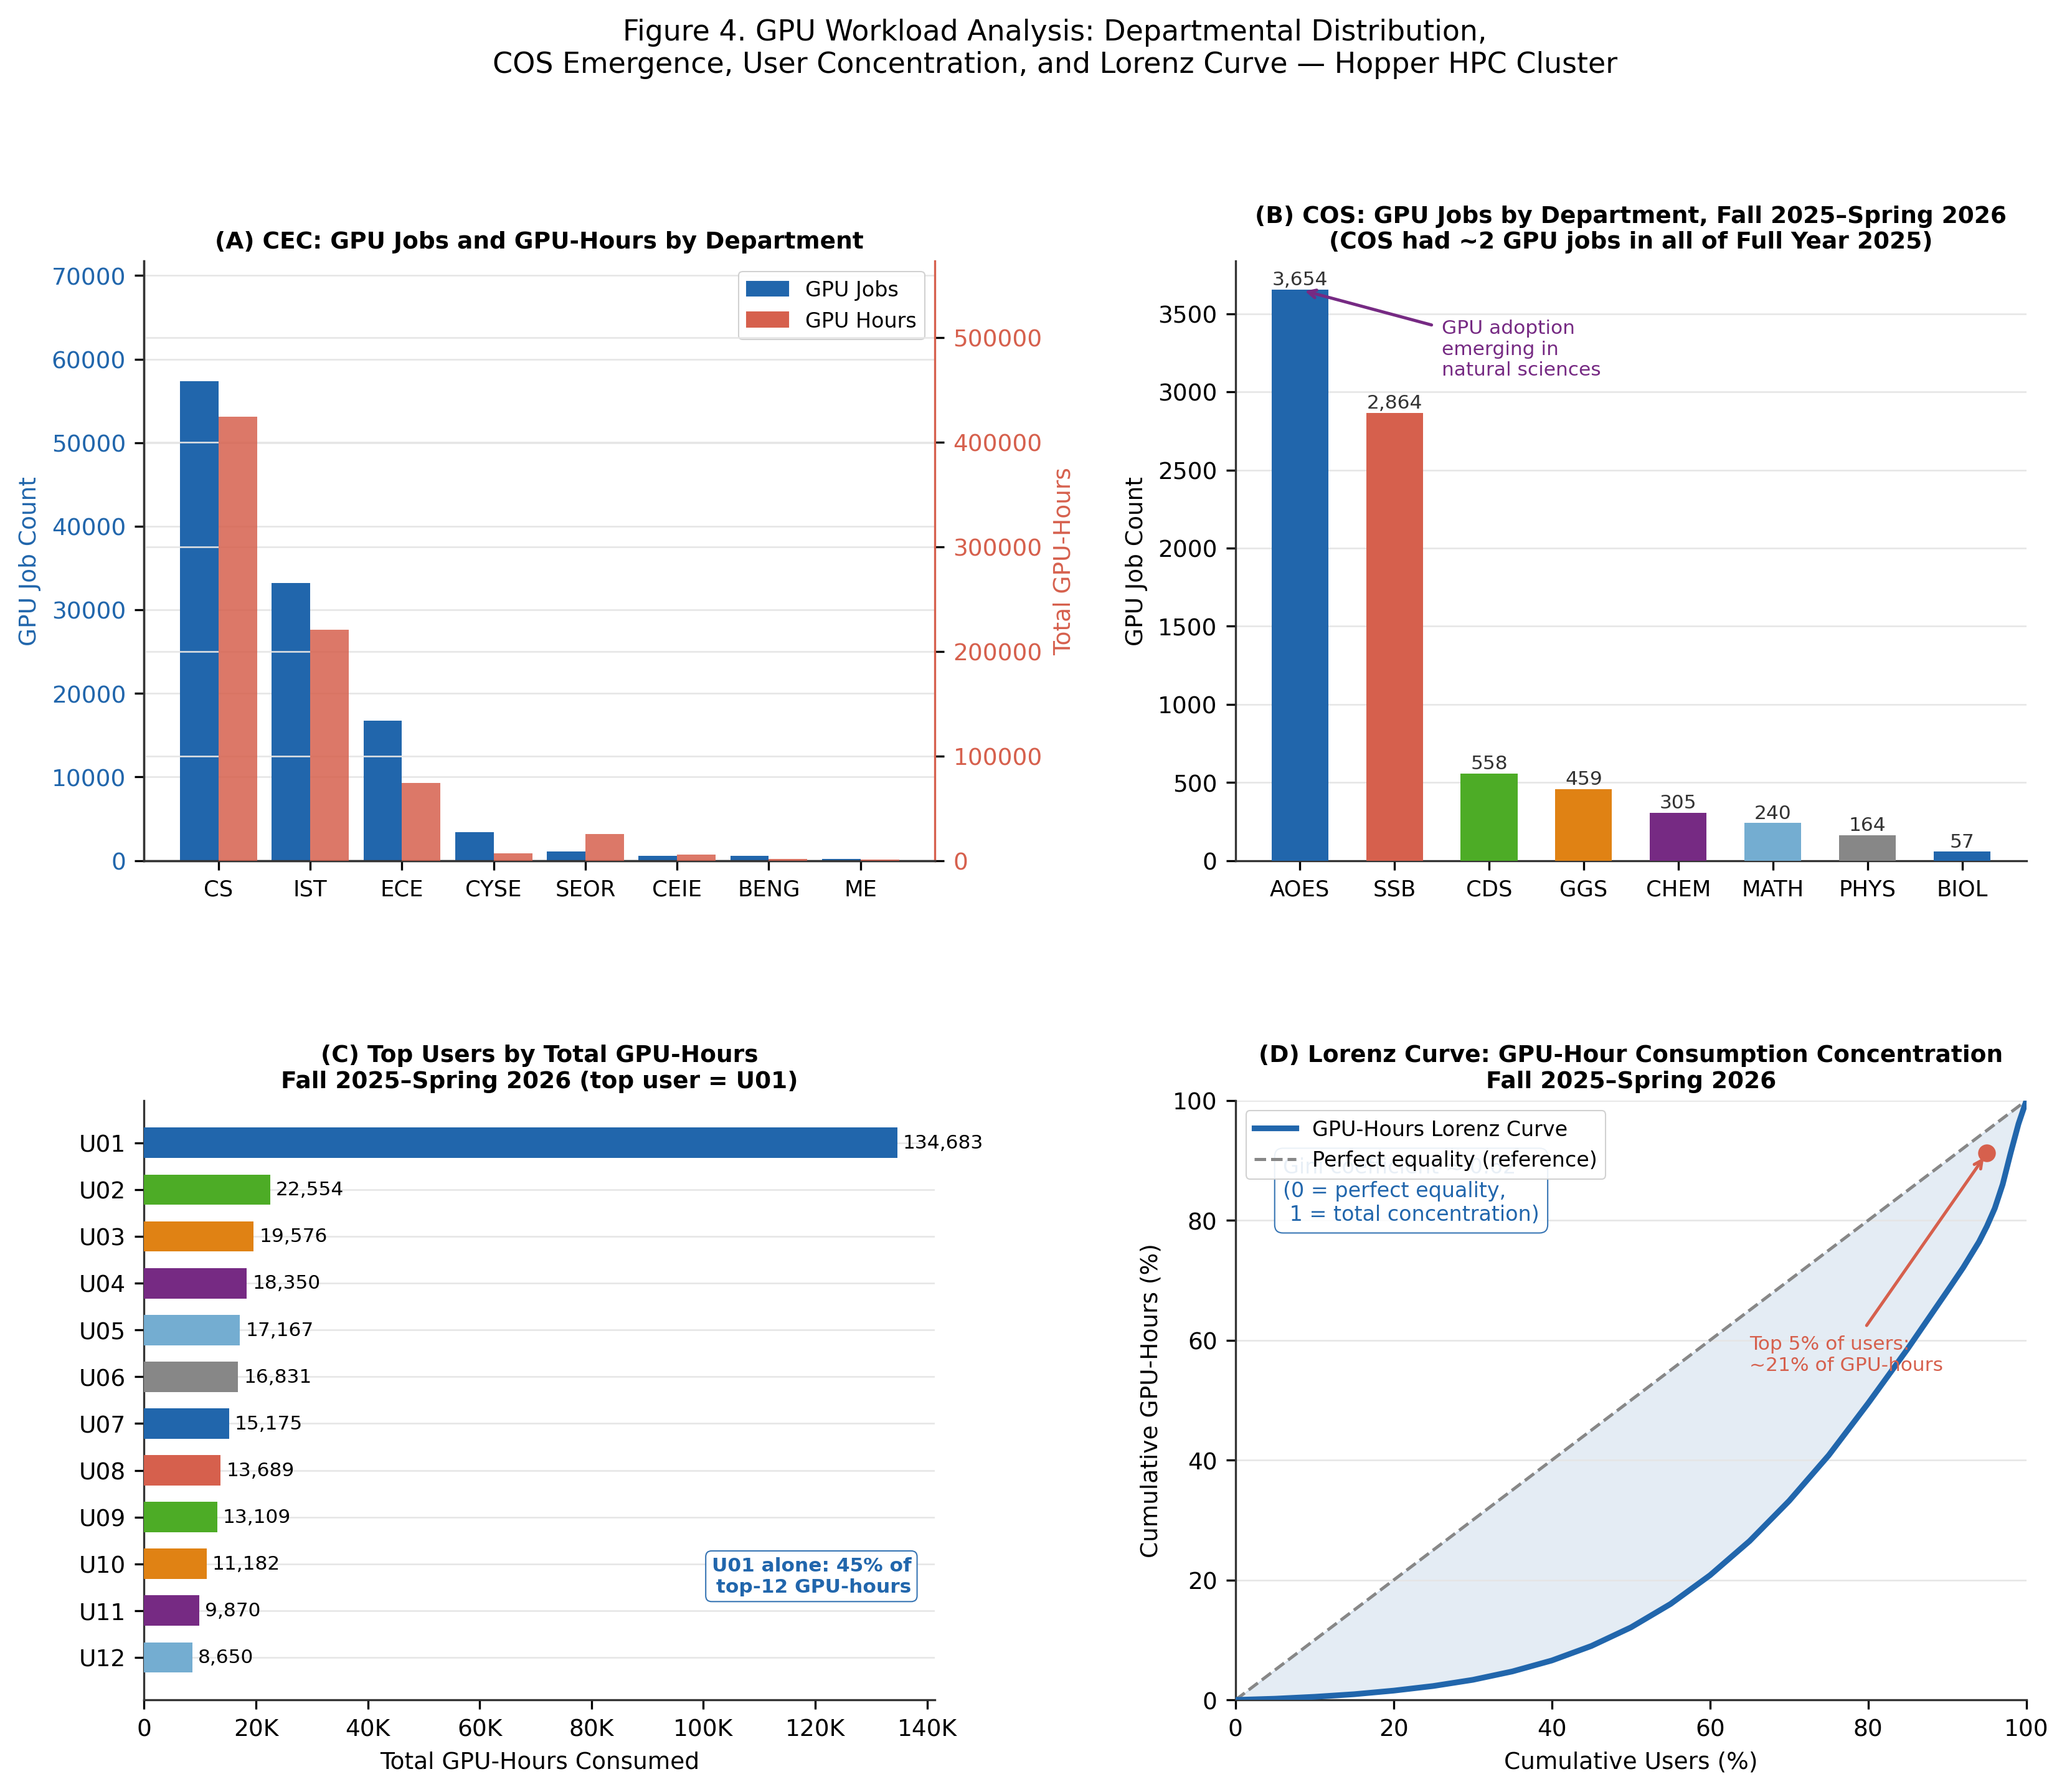
\includegraphics[width=\textwidth]{figures/fig4_gpu_analysis.png}
  \caption{GPU workload analysis, Fall~2025--Spring~2026.
    \textbf{(A)}~CEC GPU jobs and GPU-hours by department (dual y-axis).
    \textbf{(B)}~COS GPU jobs by department; the subtitle notes that COS
      submitted only $\sim$2 GPU jobs in all of Full Year~2025.
    \textbf{(C)}~Top~12 users by total GPU-hours consumed (anonymised as
      U01--U12); U01 alone accounts for 45\,\% of the top-12 total.
    \textbf{(D)}~Lorenz curve of GPU-hour consumption; the shaded area
      between the curve and the equality diagonal reflects an approximate Gini
      coefficient of 0.62.}
  \label{fig:gpu}
\end{figure}

Table~\ref{tab:top_users} presents the top GPU users by total GPU-hours.

\begin{table}[H]
  \centering
  \caption{Top users by total GPU-hours, Fall~2025--Spring~2026.
    All user identifiers are anonymised.}
  \label{tab:top_users}
  \small
  \begin{tabularx}{\textwidth}{l R{2.4cm} R{2.0cm} R{2.4cm} R{2.6cm}}
    \toprule
    \textbf{User ID} & \textbf{Total GPU Hrs} & \textbf{GPU Jobs} &
    \textbf{Avg GPU Hrs/Job} & \textbf{Avg GPU Mem (GB)} \\
    \midrule
    U01 & 134,683 & $\sim$2,513 & $\sim$54  & 392.5 \\
    U02 &  22,554 & $\sim$2,875 & $\sim$8   &  64.8 \\
    U03 &  19,576 &    $\sim$271 & $\sim$72  & 363.1 \\
    U04 &  18,350 &   5,233     &   3.5     &  39.9 \\
    U05 &  17,167 &    $\sim$241 & $\sim$71  & 304.6 \\
    U06 &  16,831 &    $\sim$196 & $\sim$86  & 429.1 \\
    \bottomrule
  \end{tabularx}
\end{table}

The concentration of GPU-hours in the top user is extreme: U01 alone consumed
more GPU-hours in the nine-month window than all COS departments combined.
This pattern is consistent with findings at comparable European HPC
facilities~\citep{netti2019}, where the top 10--15\,\% of users account for
60--80\,\% of GPU-hours.

\subsection{Instructional Utilisation}
\label{sec:instructional}

Figure~\ref{fig:instructional} presents four panels characterising instructional
GPU use, and Table~\ref{tab:instructional} lists the top accounts by job count.

\begin{figure}[H]
  \centering
  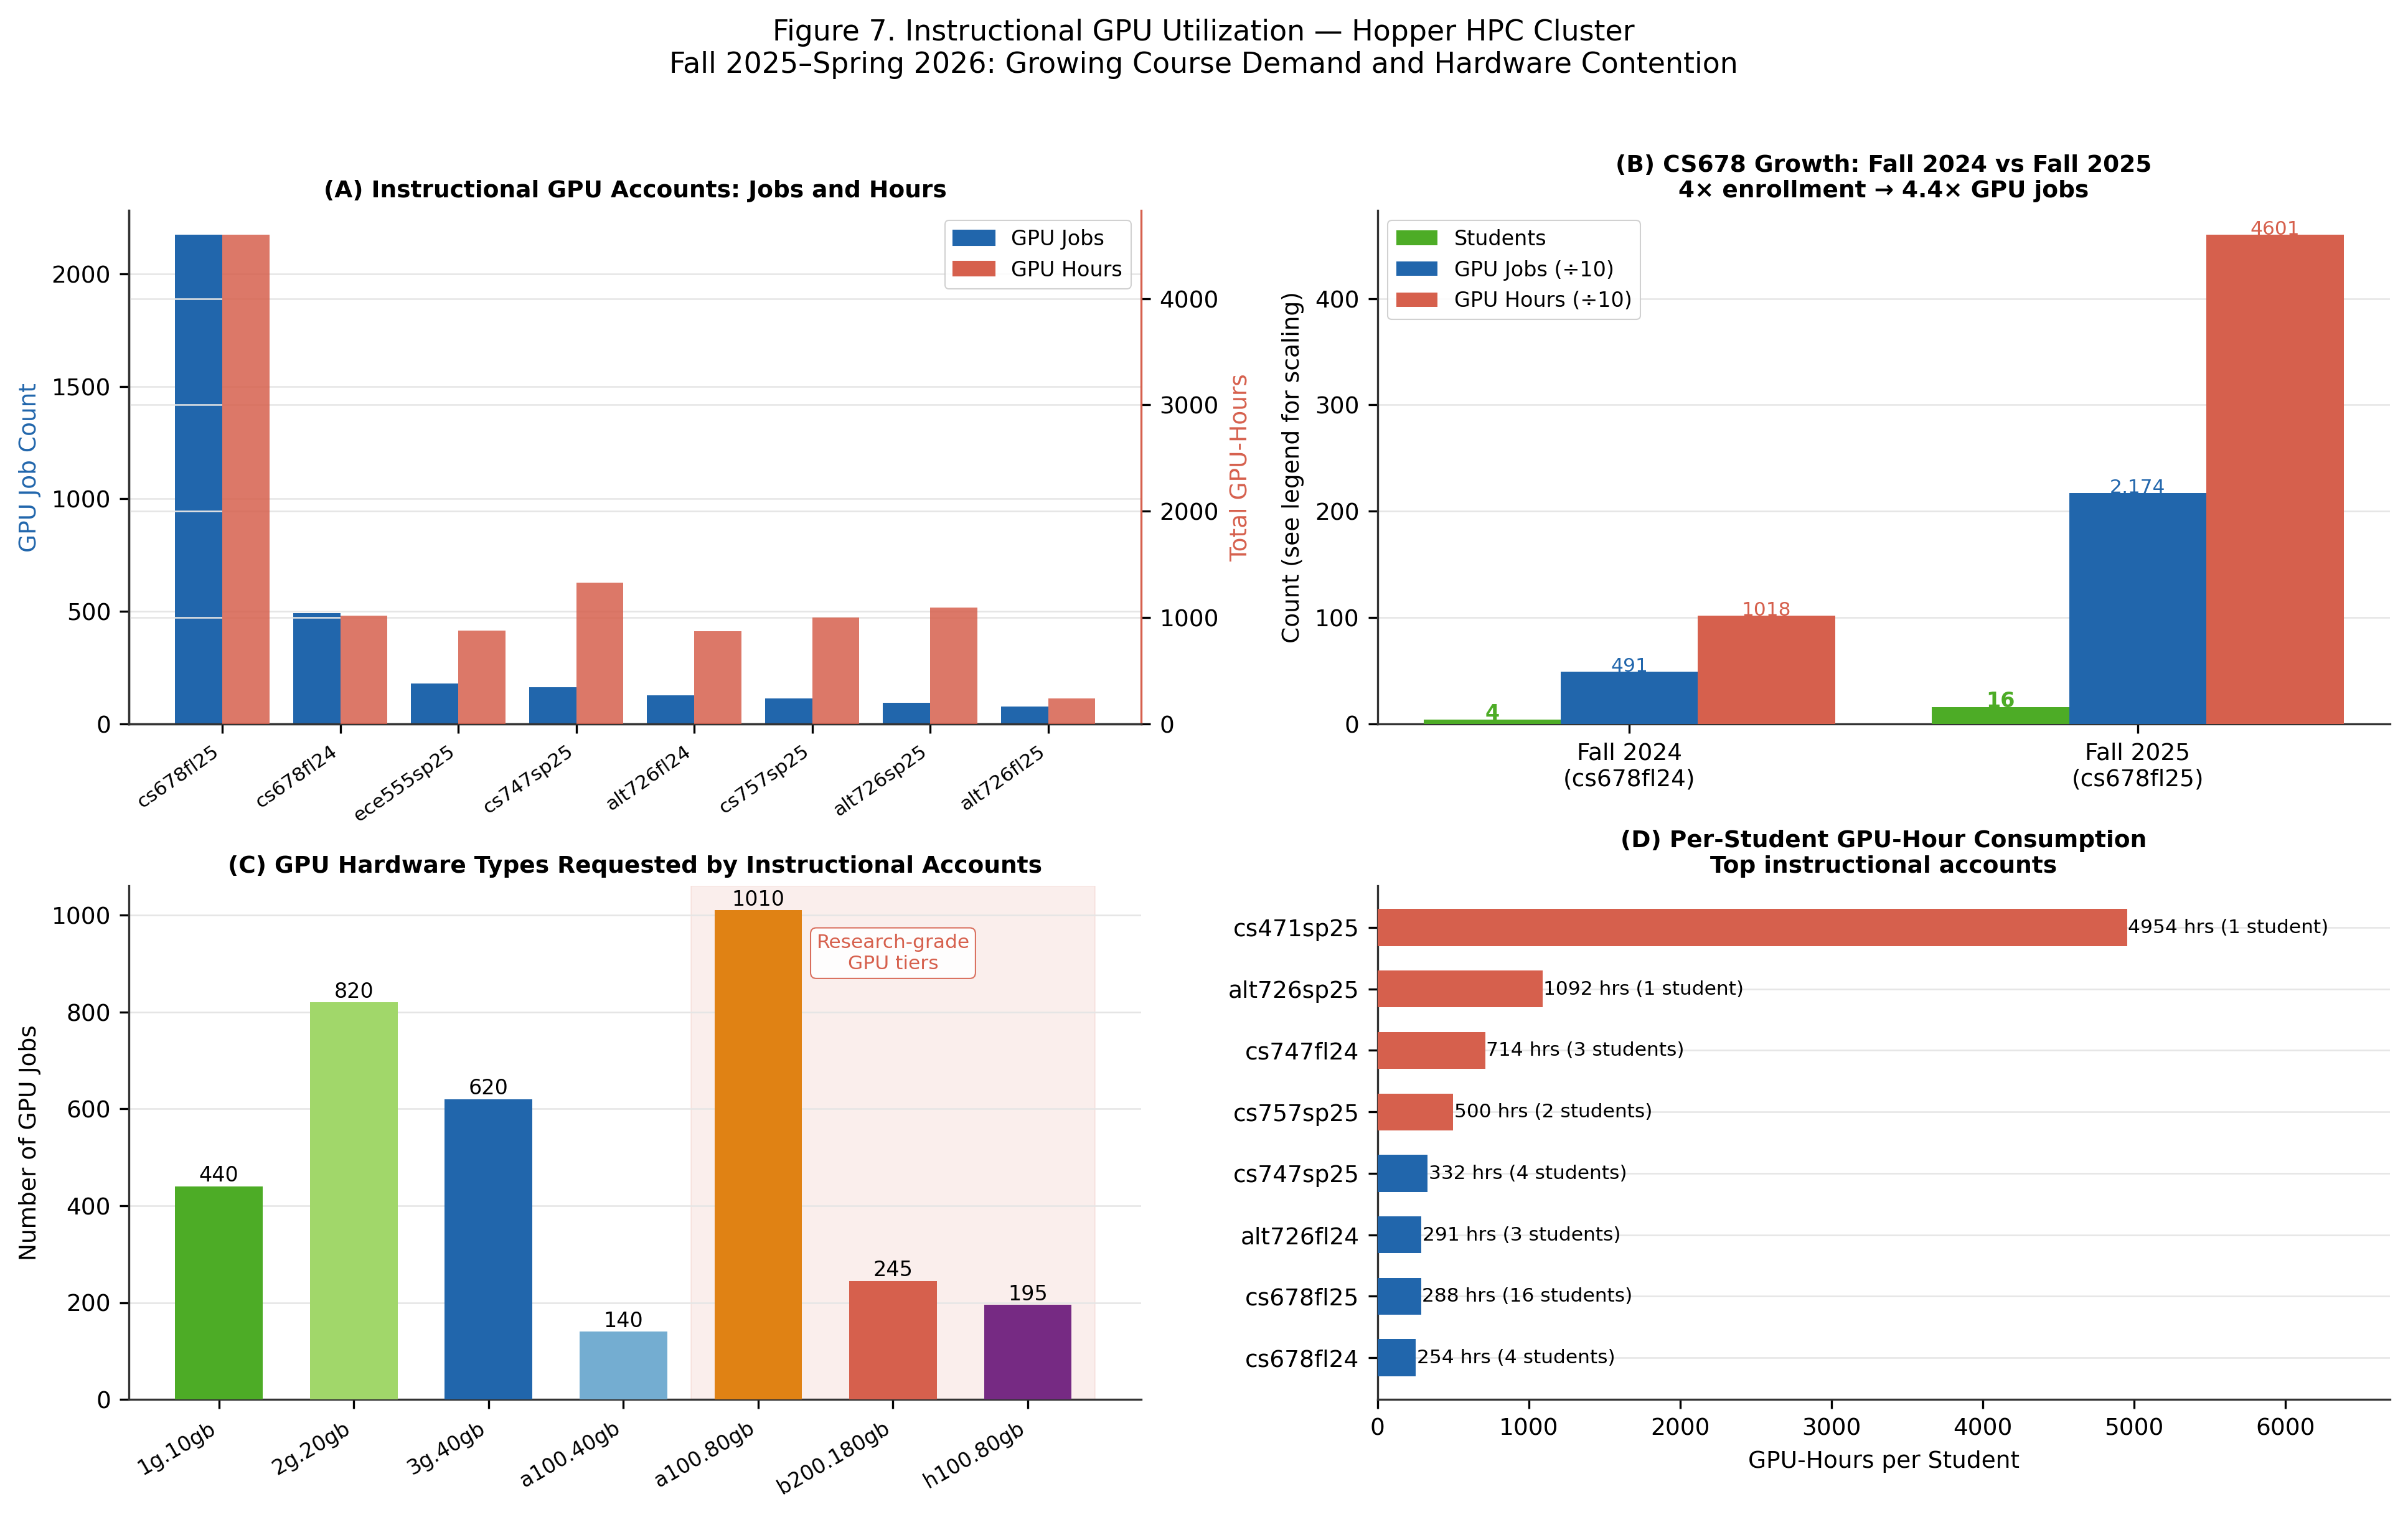
\includegraphics[width=\textwidth]{figures/fig7_instructional_gpu.png}
  \caption{Instructional GPU utilisation, Fall~2025--Spring~2026.
    \textbf{(A)}~Top instructional accounts by GPU jobs and GPU-hours.
    \textbf{(B)}~Year-over-year growth for CS678: Fall~2024 vs.\ Fall~2025,
      showing 4$\times$ enrollment driving 4.4$\times$ GPU jobs.
    \textbf{(C)}~GPU hardware types requested by course accounts; note
      requests for research-grade A100~80\,GB, B200~180\,GB, and H100~80\,GB.
    \textbf{(D)}~Per-student GPU-hour consumption for top accounts.}
  \label{fig:instructional}
\end{figure}

\begin{table}[H]
  \centering
  \caption{Top instructional GPU accounts by job count, Fall~2025--Spring~2026.
    The final row provides the preceding year's CS678 record for comparison.}
  \label{tab:instructional}
  \small
  \begin{tabularx}{\textwidth}{l R{1.6cm} R{1.6cm} R{2.0cm} R{2.8cm}}
    \toprule
    \textbf{Account} & \textbf{Students} & \textbf{GPU Jobs} &
    \textbf{GPU Hrs} & \textbf{Avg GPU Hrs/Job} \\
    \midrule
    cs678fl25   & 16 & 2,174 & 4,601 & 2.12  \\
    alt726sp25  &  1 &    94 & 1,092 & 11.63 \\
    cs471sp25   &  1 &    72 & 4,954 & 68.81 \\
    cs747sp25   &  4 &   162 & 1,330 &  8.21 \\
    cs757sp25   &  2 &   114 & 1,001 &  8.79 \\
    \midrule
    cs678fl24\textsuperscript{†} & 4 & 491 & 1,018 & 2.07 \\
    \bottomrule
  \end{tabularx}
  \smallskip\par
  \raggedright\footnotesize \textsuperscript{†} Prior-year comparison record.
\end{table}

\subsection{CPU Request Distribution}
\label{sec:cpu_dist}

Figure~\ref{fig:cpu_dist} reveals a pronounced bimodal structure in the
distribution of CPU cores requested per job.

\begin{figure}[H]
  \centering
  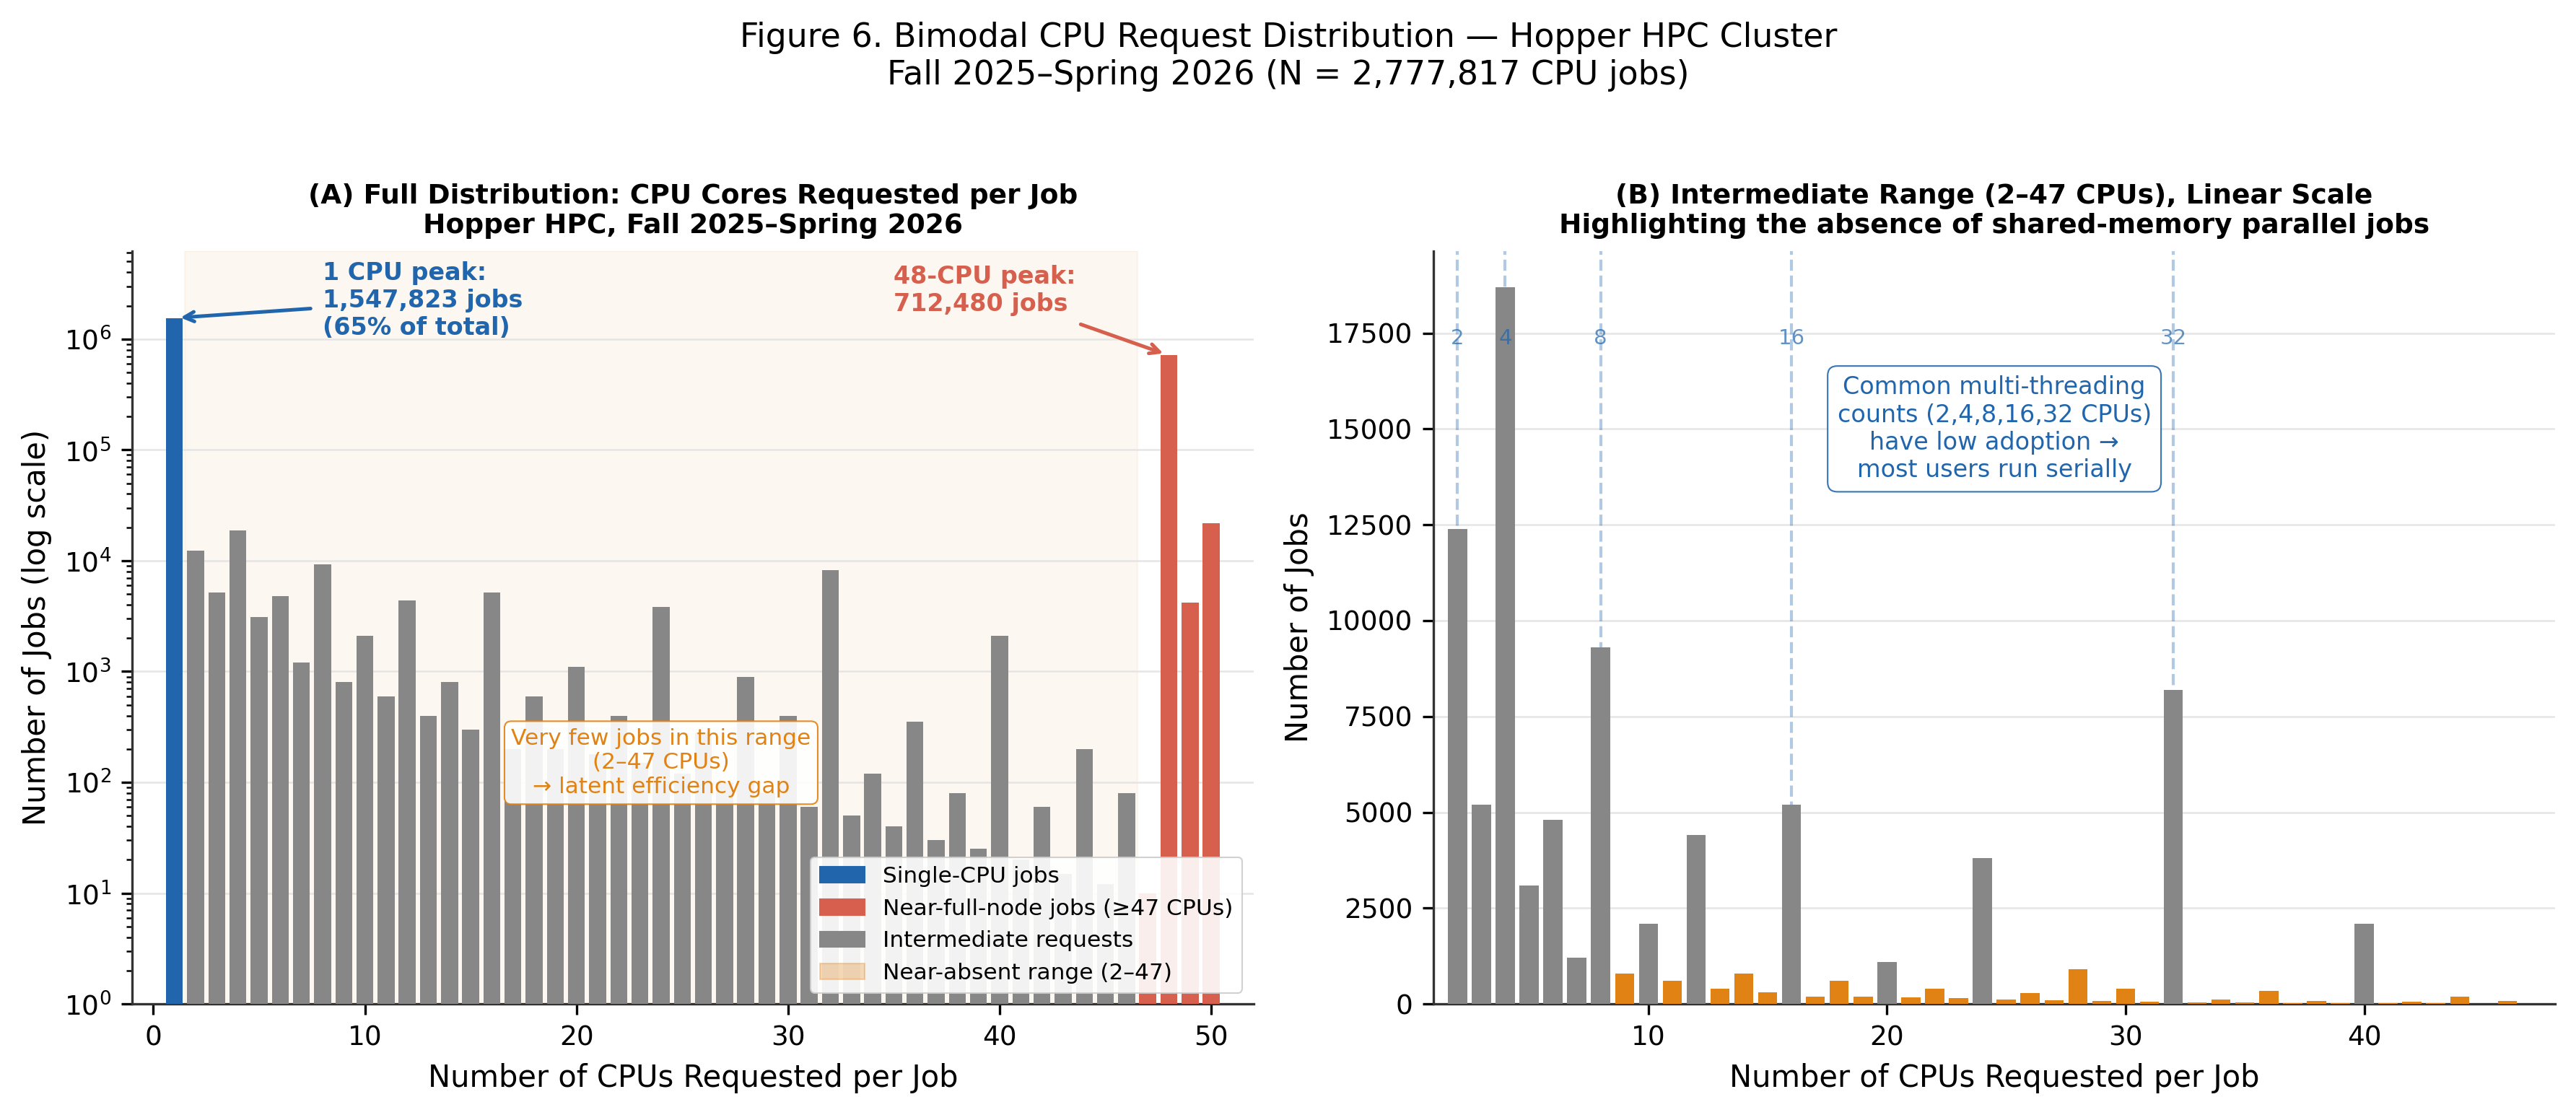
\includegraphics[width=\textwidth]{figures/fig6_cpu_distribution.png}
  \caption{Distribution of CPU cores requested per job, Fall~2025--Spring~2026
    ($N = 2{,}777{,}817$ CPU jobs).
    \textbf{(A)}~Full distribution on a logarithmic y-axis.  The dominant peak
      at 1~CPU (1,547,823 jobs; 65\,\% of total) and the secondary peak near
      48~CPUs (712,480 jobs) are highlighted.
    \textbf{(B)}~Zoomed view of the 2--47-CPU range on a linear scale,
      revealing the near-complete absence of intermediate multi-core requests.}
  \label{fig:cpu_dist}
\end{figure}

The dominant peak at 1~CPU accounts for approximately 65\,\% of all CPU jobs.
A secondary peak at 48~CPUs (approximately one full node on standard \hopper{}
configurations) contains a further 25\,\%.  The intermediate range of 2--47~CPUs
is nearly absent, indicating that most researchers either run serially or jump
directly to full-node allocations, with very little adoption of intermediate-scale
shared-memory parallelism.

\subsection{Queue Health and Temporal Patterns}
\label{sec:queue}

Figure~\ref{fig:queue} presents temporal utilisation patterns: monthly job volume
for Full Year~2025 and monthly average wait and run times for Fall~2025--Spring~2026.
Table~\ref{tab:queue} provides the numerical wait/run-time data.

\begin{figure}[H]
  \centering
  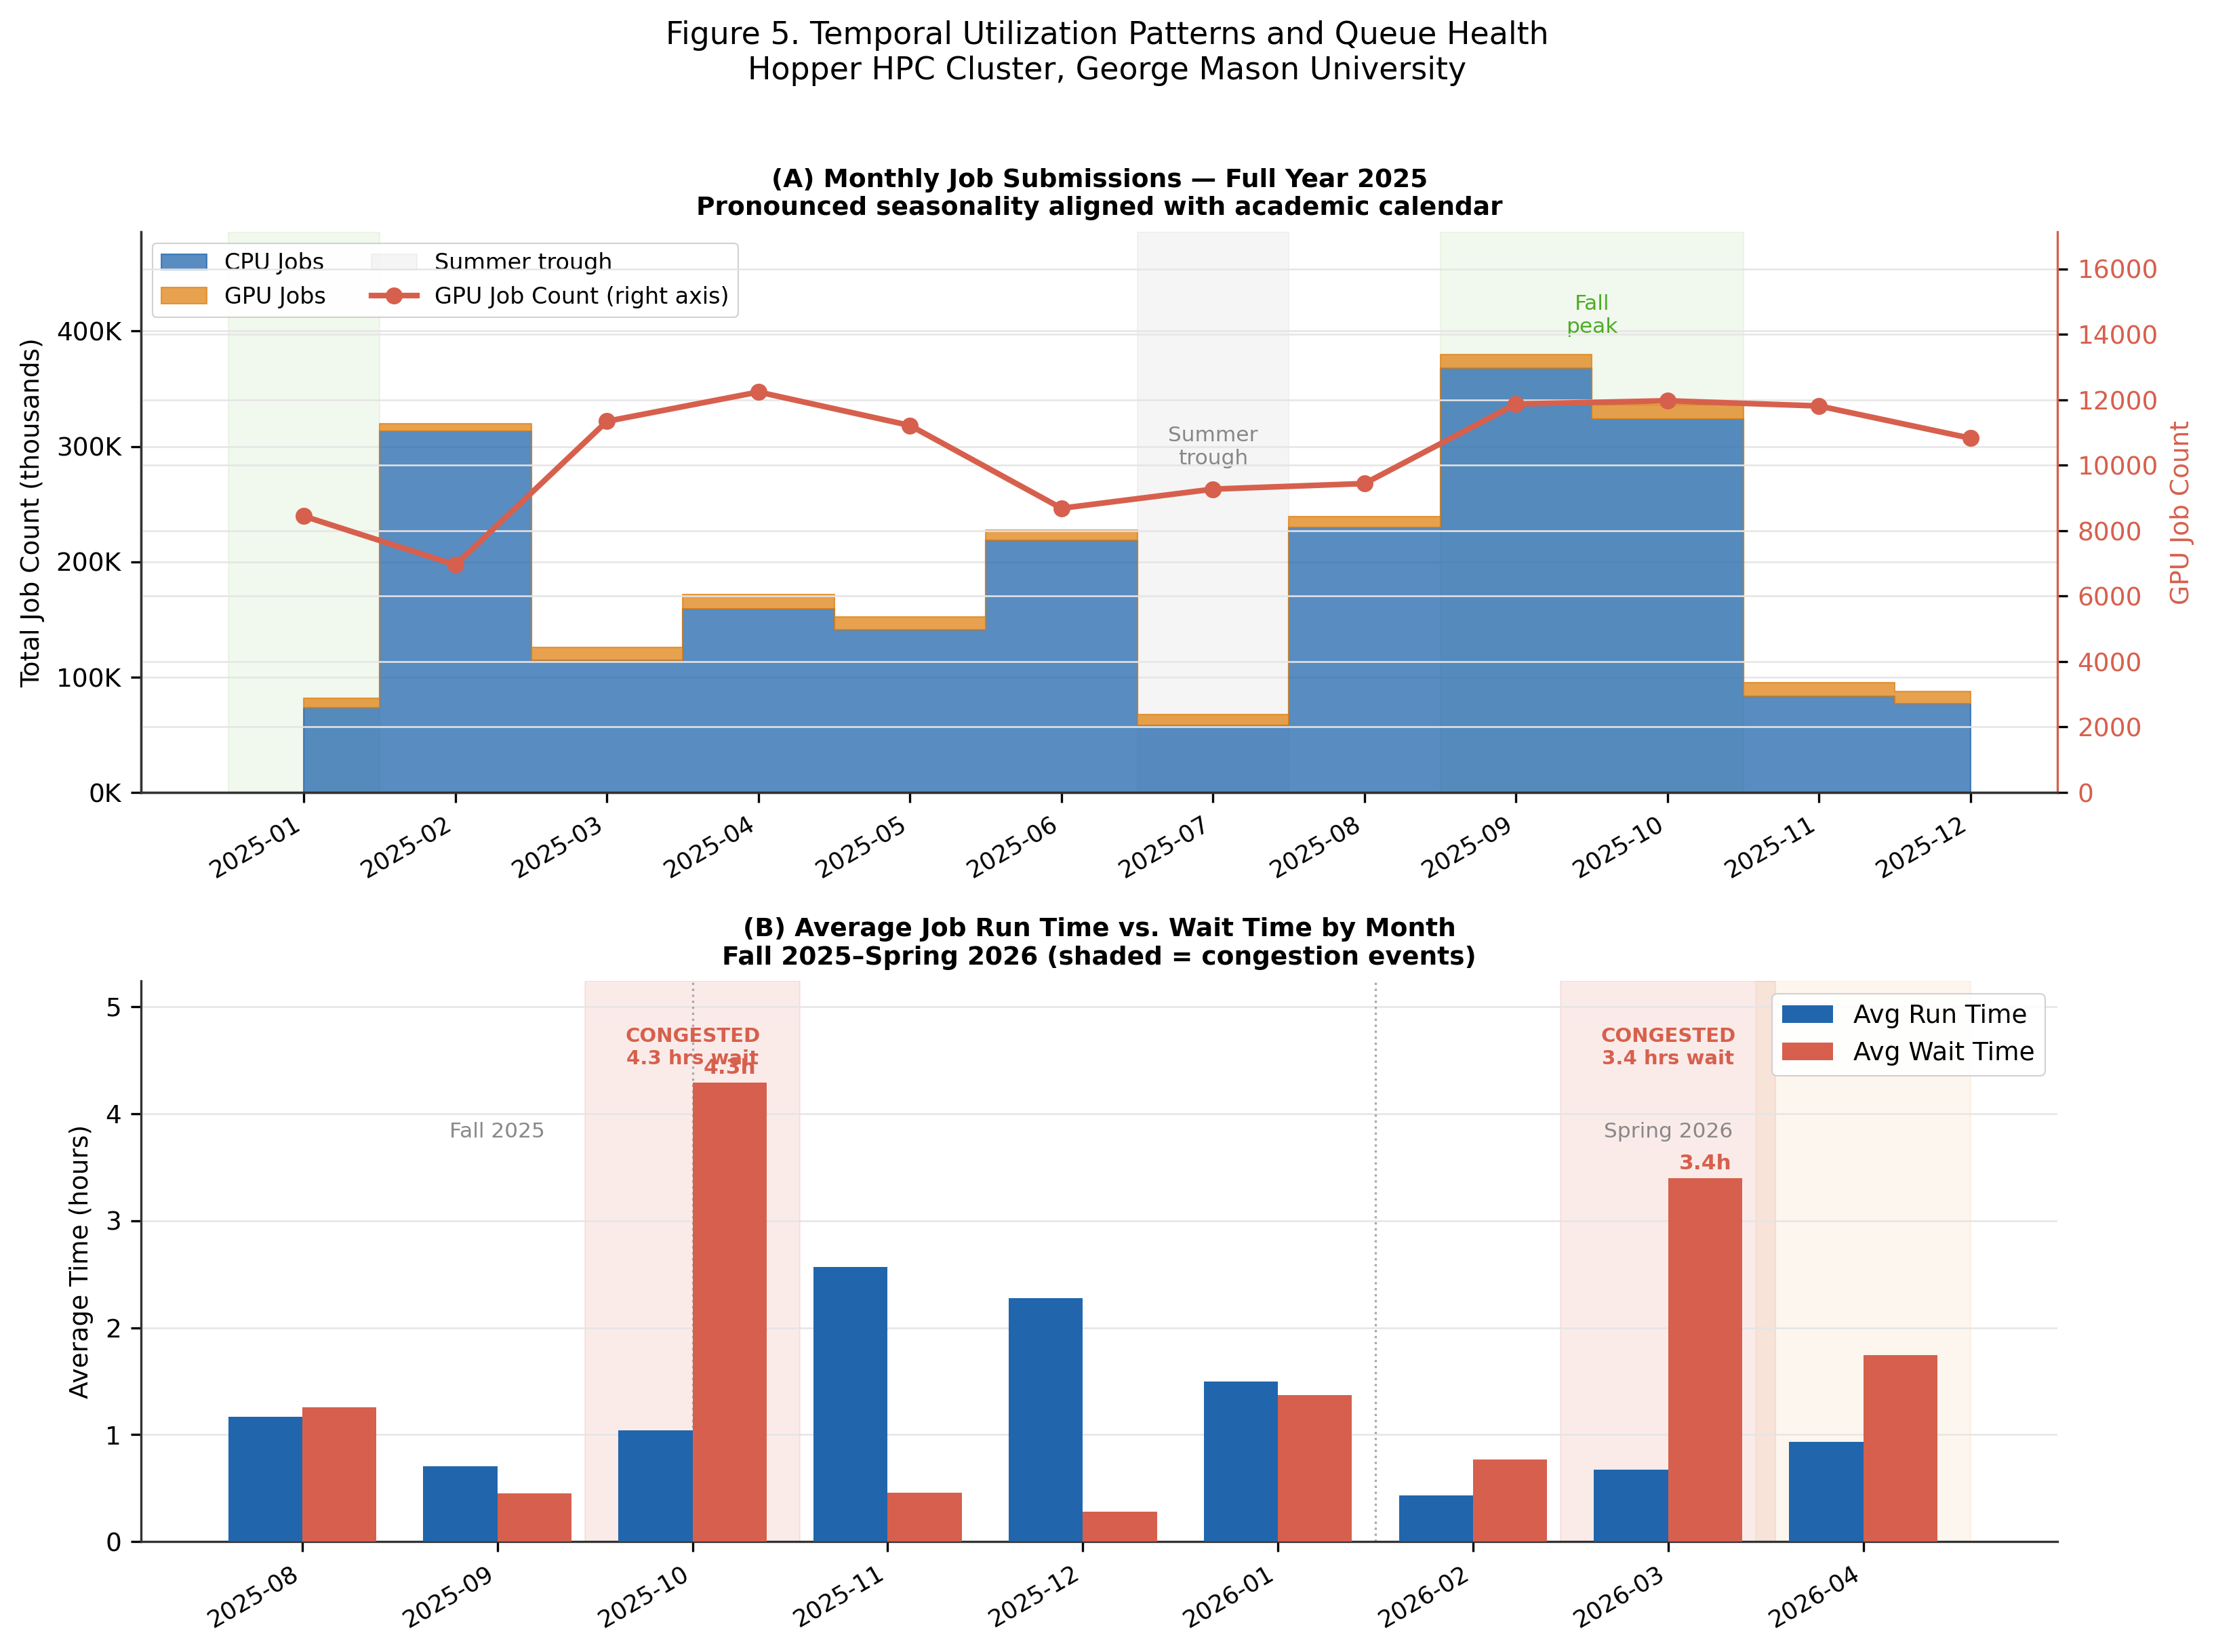
\includegraphics[width=\textwidth]{figures/fig5_queue_dynamics.png}
  \caption{Temporal utilisation patterns.
    \textbf{(A)}~Monthly CPU and GPU job submissions, Full Year~2025, with the
      summer trough and fall peak annotated.  The GPU job count trend is overlaid
      on the right axis (red line).
    \textbf{(B)}~Average job run time (blue) and wait time (red) by month,
      Fall~2025--Spring~2026.  Months classified as ``congested'' (October~2025
      and March~2026) are highlighted with a red background shade.  Vertical
      dashed lines mark the Fall~2025/Spring~2026 semester boundary.}
  \label{fig:queue}
\end{figure}

\begin{table}[H]
  \centering
  \caption{Monthly average run time and wait time, Fall~2025--Spring~2026.}
  \label{tab:queue}
  \small
  \begin{tabularx}{0.72\textwidth}{l R{2.8cm} R{2.8cm} l}
    \toprule
    \textbf{Month} & \textbf{Avg Run (hrs)} & \textbf{Avg Wait (hrs)} &
    \textbf{Status} \\
    \midrule
    2025-08 & 1.17 & 1.25 & Normal \\
    2025-09 & 0.71 & 0.45 & Low    \\
    2025-10 & 1.04 & \textbf{4.29} & \textbf{Congested} \\
    2025-11 & 2.56 & 0.46 & Normal \\
    2025-12 & 2.28 & 0.28 & Low    \\
    2026-01 & 1.50 & 1.37 & Normal \\
    2026-02 & 0.43 & 0.77 & Normal \\
    2026-03 & 0.68 & \textbf{3.40} & \textbf{Congested} \\
    2026-04 & 0.93 & 1.74 & Elevated \\
    \bottomrule
  \end{tabularx}
\end{table}

Two months exhibit substantially elevated average wait times:
October~2025 (4.29~hours) and March~2026 (3.40~hours), corresponding to
predictable points in the academic calendar: the first major research crunch
of each semester.

Figure~\ref{fig:users} presents daily active users and the CEC IST outlier
profile.

\begin{figure}[H]
  \centering
  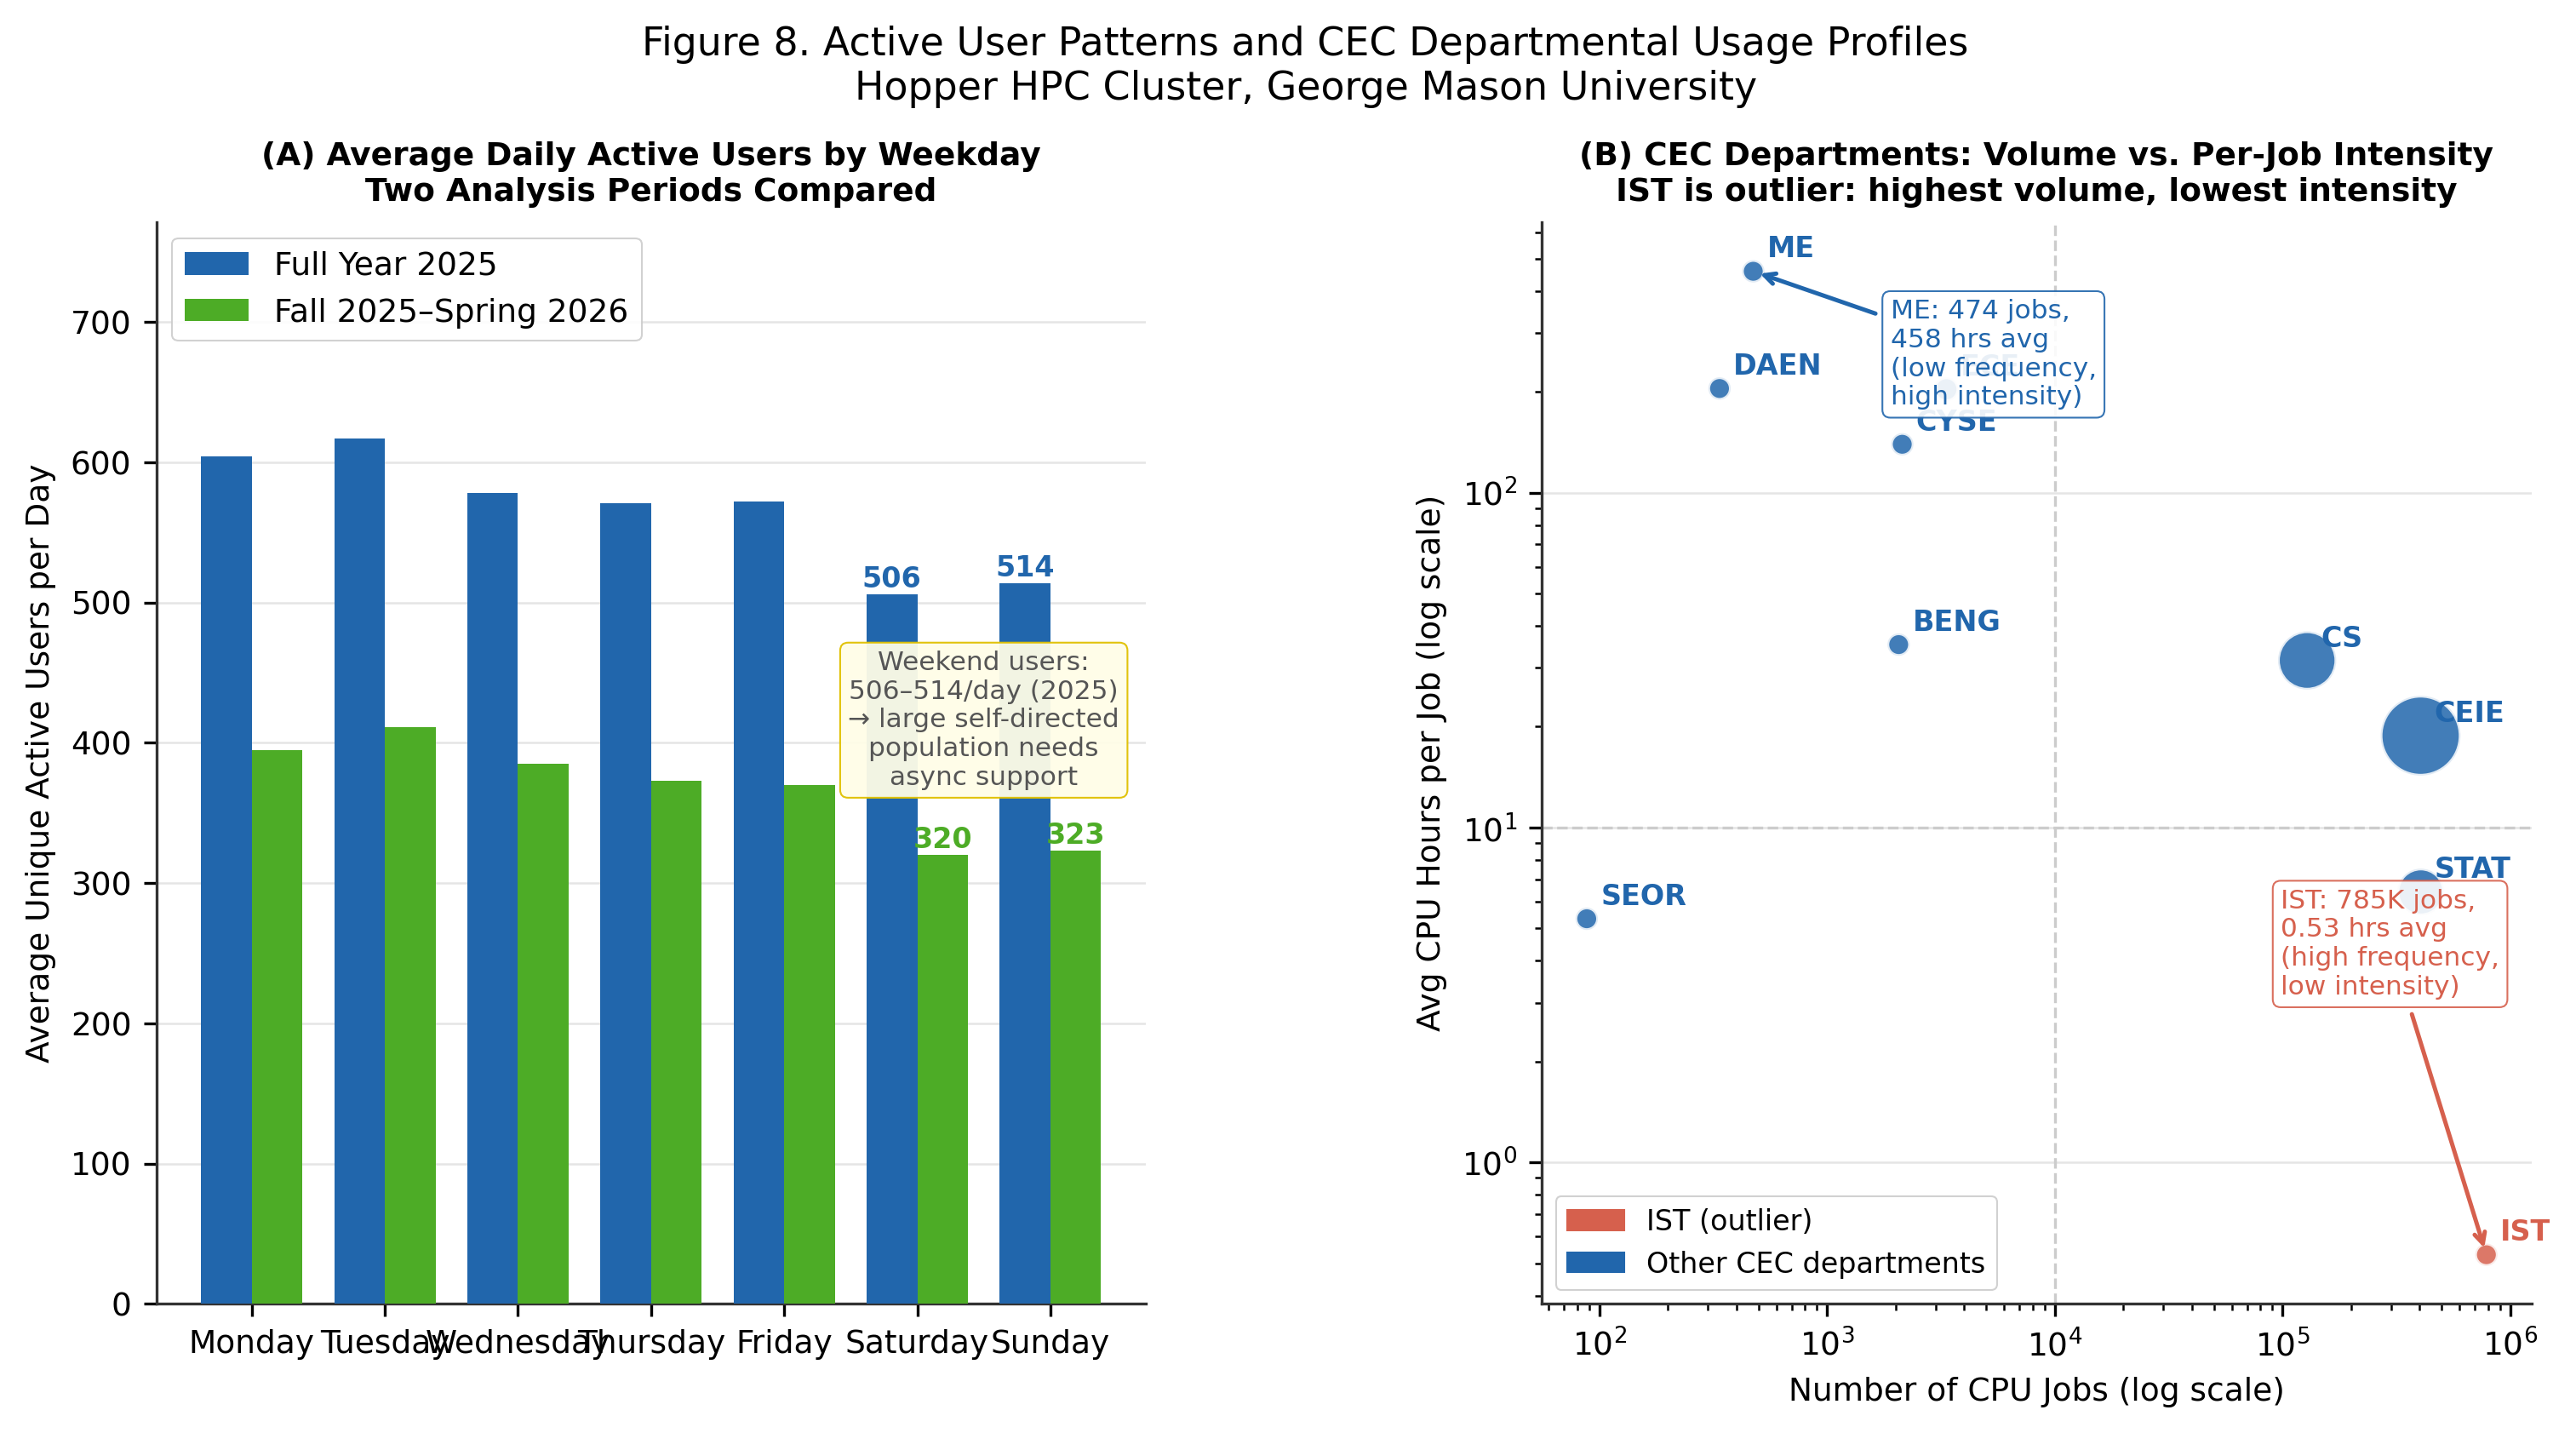
\includegraphics[width=\textwidth]{figures/fig8_active_users.png}
  \caption{Active user patterns and CEC departmental usage profiles.
    \textbf{(A)}~Average unique daily active users by day of week, comparing
      Full Year~2025 (blue) and Fall~2025--Spring~2026 (green).  Weekend counts
      of 320--514 users per day confirm a large self-directed user population.
    \textbf{(B)}~CEC departments plotted by CPU job count (x-axis) vs.\
      average CPU-hours per job (y-axis), both on logarithmic scales.  IST
      (highlighted in red) is a clear outlier: the highest volume department
      with the lowest per-job intensity.  Bubble area is proportional to total
      CPU-hours consumed.}
  \label{fig:users}
\end{figure}

%% ====================================================================
\section{Discussion}
\label{sec:discussion}

\subsection{A Structurally Transformed User Community}

The data collectively indicate that the \hopper{} user community has undergone a
structural transformation, not merely quantitative growth.  IST's emergence as
the largest job submitter---with a usage profile that differs categorically from
all other major departments---is the clearest illustration of this diversity.
IST's workload appears driven by automated analysis pipelines, classroom
exercises, or workflow frameworks generating thousands of short jobs rather than
the intensive long-running computations traditionally associated with HPC.  From
a scheduling perspective, IST's workload is not particularly resource-intensive;
but thousands of short jobs submitted in bursts can inflate queue length and
interfere with fair scheduling for users submitting fewer but larger jobs.

\subsection{The GPU Transition: Acceleration, Concentration, and Spillover}

GPU utilisation has entered a new phase characterised by three concurrent
developments: overall demand growth, extreme user-level concentration, and
cross-disciplinary spillover into natural science fields.  GPU daily job counts
roughly quadrupled between early 2025 and Spring~2026.  A single user consuming
more GPU-hours than the next six combined constitutes a structural inequity that
conventional first-come, first-served scheduling cannot address.  The emergence
of GPU workloads in COS---essentially zero in 2025, approximately 8,300~jobs by
Spring~2026---represents the earliest phase of a GPU adoption curve in the natural
sciences, with atmospheric modelling, protein structure prediction, and ML
interatomic potentials as the leading applications.

\subsection{Instructional GPU Demand and Hardware Contention}

Students in CS678, CS471, and similar courses are requesting access to A100~80\,GB,
H100, and B200 hardware that is simultaneously the most demanded resource for
research GPU users.  The increase in CS678 enrolment from 4~students in
Fall~2024 to 16~students in Fall~2025---a 4$\times$ increase in a single
year---suggests that instructional GPU demand is not simply growing but
accelerating.  Without a hardware partitioning strategy, the conflict between
instructional and research GPU use will intensify predictably with each semester.

\subsection{The Bimodal CPU Distribution as a Latent Efficiency Opportunity}

The near-complete absence of jobs requesting 2--47~CPUs is unusual and warrants
attention beyond its statistical interest.  OpenMP, Python multiprocessing, and
R parallel computing frameworks can provide 4--16$\times$ speedups for many common
workflows with minimal code modification.  Targeted training in intermediate-scale
parallelism for IST and STAT populations---the departments with the largest
numbers of single-CPU job submitters---represents a high-leverage, low-cost
intervention.

\subsection{Semester-Synchronised Congestion}

The October and March wait-time spikes (4.29 and 3.40~hours, respectively) are
predictable consequences of semester-correlated research activity and are unlikely
to resolve through organic scheduling behaviour.  Proactive queue management---
coordinated advance notice to the heaviest users before congestion events
materialise---is a well-established intervention in operational HPC
support~\citep{ragavan2020}.

%% ====================================================================
\section{Data-Driven Interventions}
\label{sec:interventions}

\subsection{Personnel Specialisation}

The scale and complexity of GPU workloads now justify a dedicated \textbf{GPU
Specialist} within the \orc{} researcher-facing staff, requiring deep competency
in CUDA, distributed GPU training frameworks (PyTorch DDP, JAX pmap, DeepSpeed),
GPU memory profiling (DCGM, Nsight), and containerised GPU environments.  The
COS utilisation growth and GPU emergence requires a dedicated \textbf{COS
Liaison} with competency in domain workflows: WRF/MOM6, GROMACS/NAMD/AMBER,
AlphaFold, and geospatial computing.  Given that IST generates more job records
than any other department, an \textbf{IST/CS Instructional Coordinator} focused
on semester-start onboarding, SLURM template development, and per-course quota
planning would have disproportionate impact.

\subsection{Queue and Scheduling Policy}

We recommend a per-user GPU-hour soft cap on a rolling window
(e.g., 10,000~GPU-hours per week), above which jobs receive lower scheduling
priority rather than being blocked.  Course accounts should be restricted to
lower-tier GPU partitions (1g.10gb, 2g.20gb, 3g.40gb via MIG) unless documented
educational justification for high-memory devices is approved.  Jobs requesting
more than 512~CPUs, 72~hours of wall time, or 2~TB of memory should require a
pre-submission consultation.  Proactive semester-aligned outreach to the top
100~job submitters two weeks before each predicted congestion event (early October,
mid-March) should be implemented as a standing operational procedure.

\subsection{Infrastructure Planning}

At current growth rates, GPU queue pressure will become a chronic operational
constraint within one to two academic years.  Hardware procurement should
prioritise additional A100~80\,GB or H100~80\,GB nodes for research, with MIG
partitioning for instructional access.  The large memory demands in AOES
(254\,GB avg) and GGS (228\,GB avg) suggest the high-memory node pool should be
assessed for adequacy.  Open OnDemand additions immediately justified by the data
include GPU-enabled Jupyter environments and an interactive GPU session option for
debugging.

\subsection{Outreach and Training}

A focused half-day workshop targeting IST and STAT users on Python multiprocessing,
joblib, and array-job frameworks would address the bimodal CPU distribution at
scale.  COS GPU onboarding should begin now, targeting AOES (JAX for atmospheric
modelling, neural-network potentials) and SSB (AlphaFold, genomic deep learning)
while these communities are in early adoption.

%% ====================================================================
\section{Job Failure Rate Analysis}
\label{sec:failure}

This section presents analysis A2: a systematic examination of job exit states,
the wasted compute resources attributable to failure modes, and the relationship
between job failure rates and queue congestion.

\subsection{Exit-State Distribution by Department}

Figure~\ref{fig:failure} presents four panels characterising job failure patterns
across departments and time.  Panel~A shows the percentage breakdown of exit
states for the nine highest-volume departments in Fall~2025--Spring~2026.

\begin{figure}[H]
  \centering
  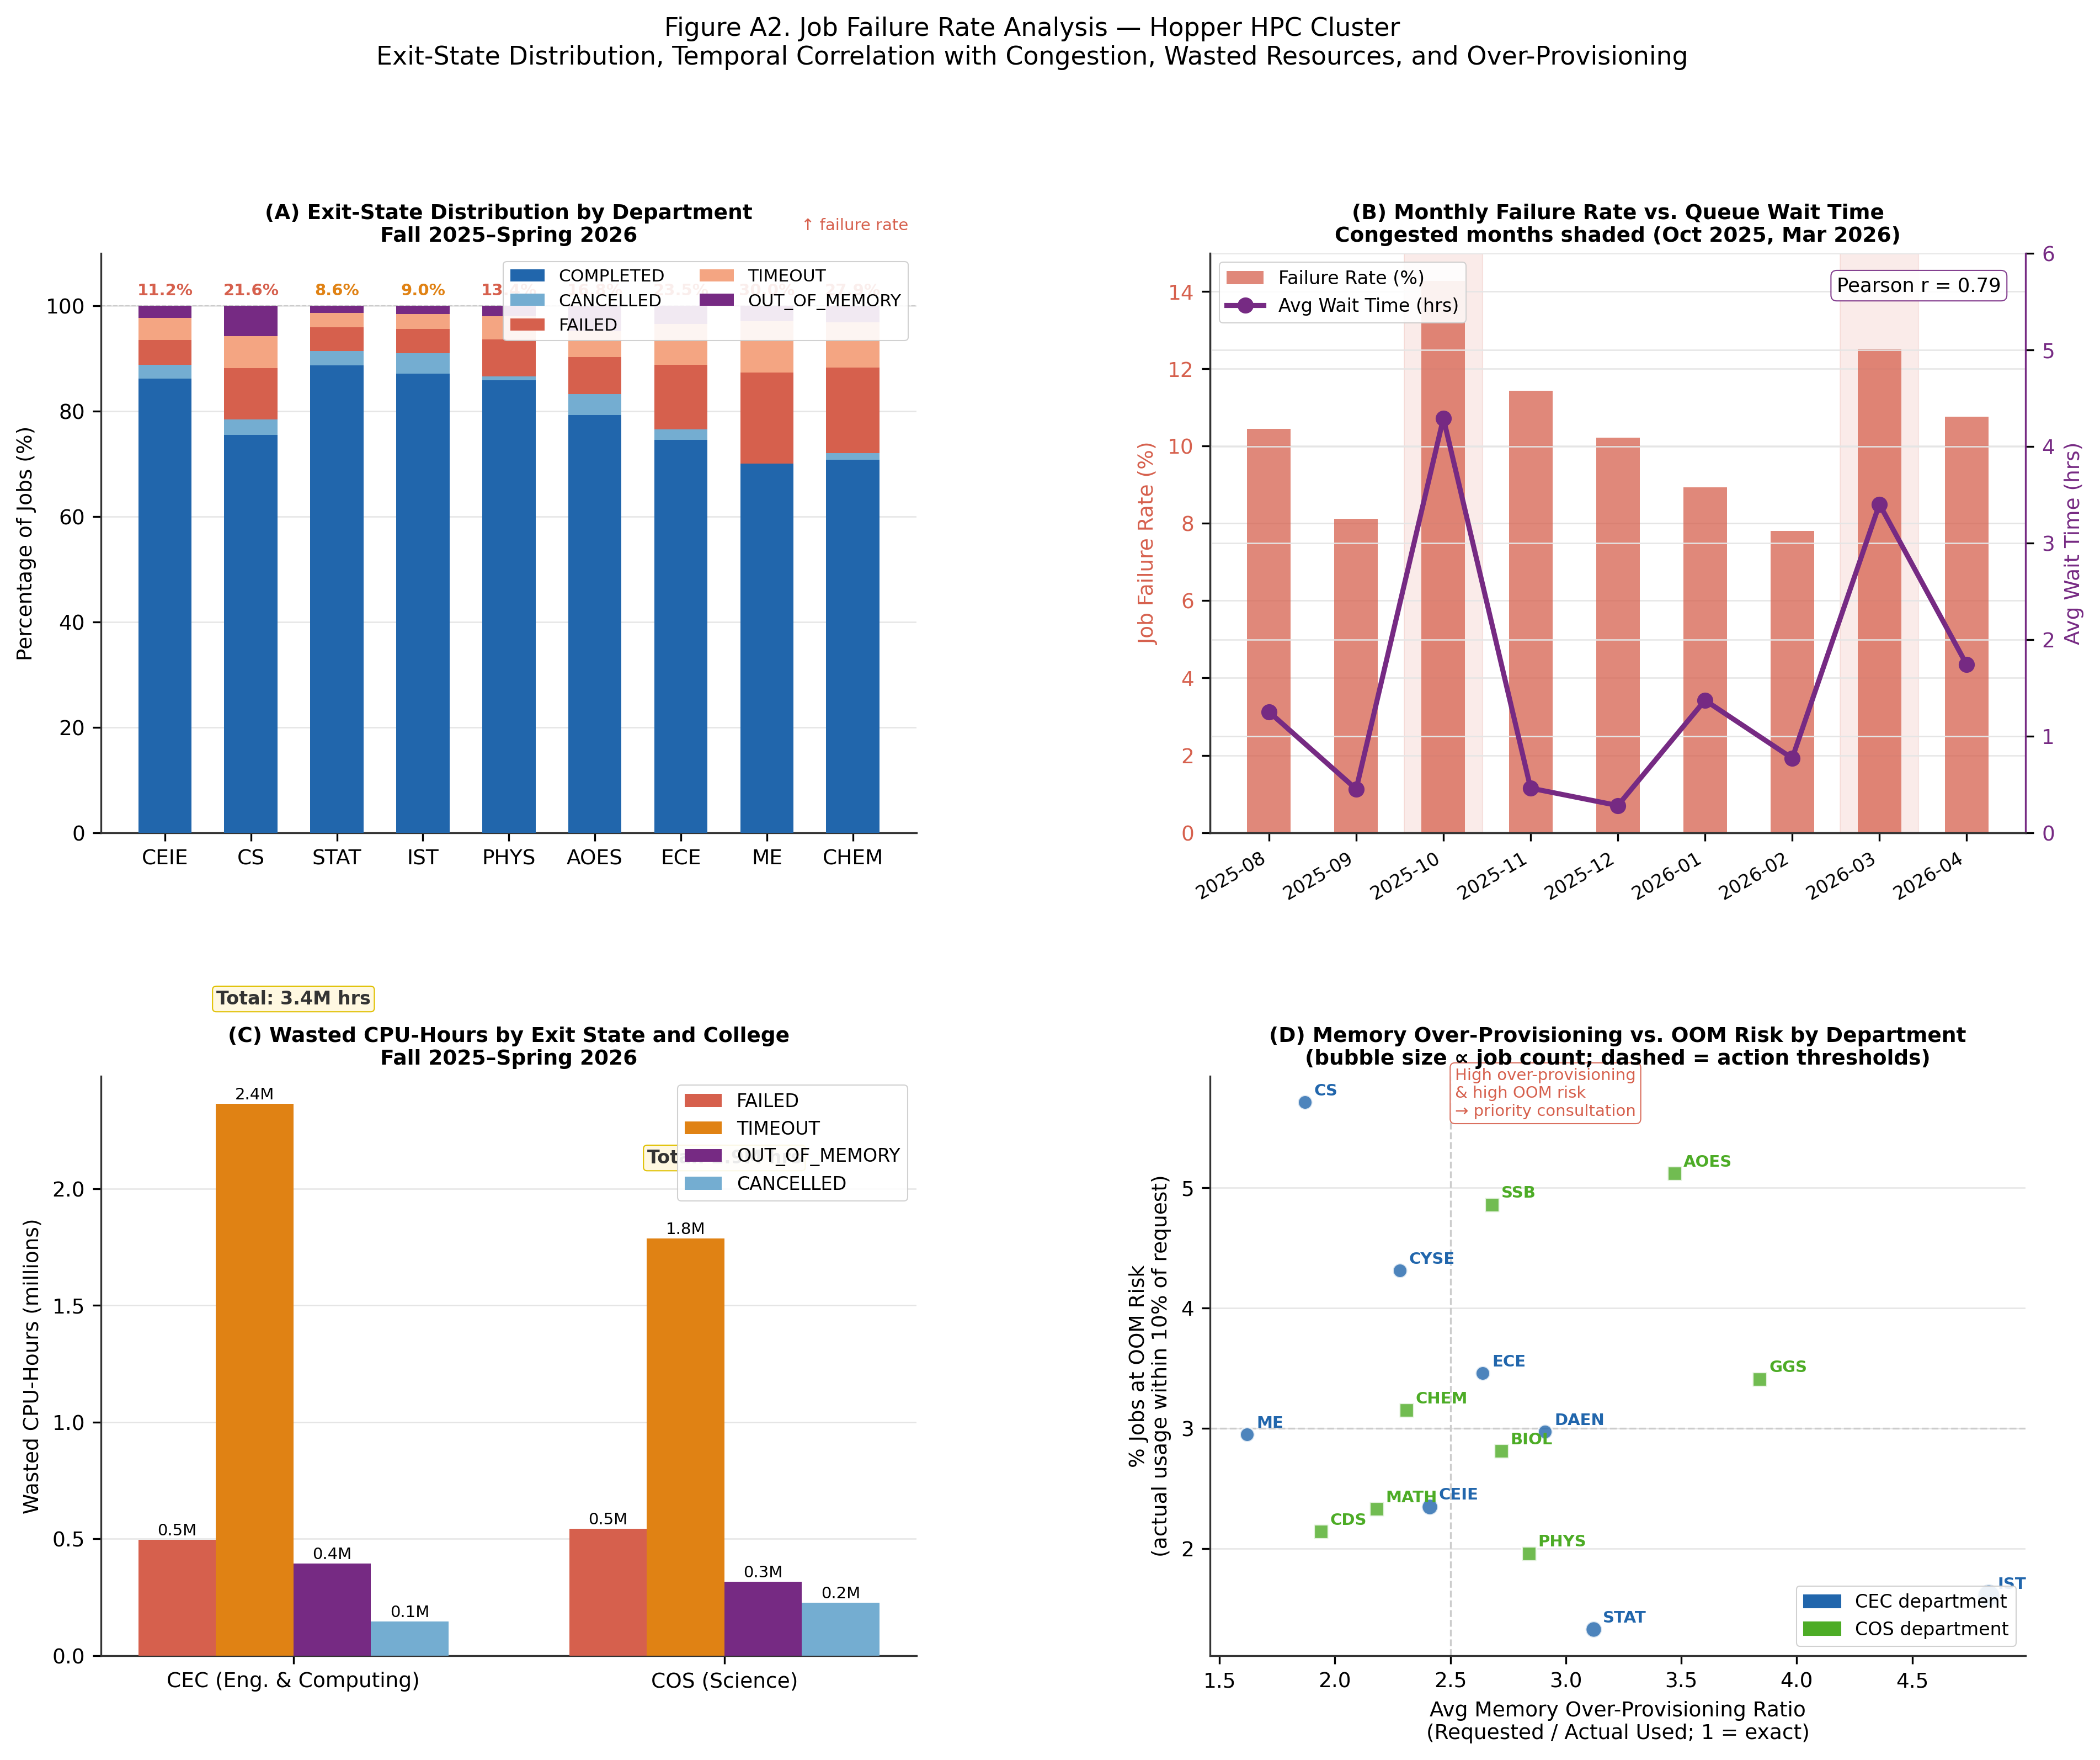
\includegraphics[width=\textwidth]{figures/figA2_failure_analysis.png}
  \caption{Job failure rate analysis, Fall~2025--Spring~2026.
    \textbf{(A)}~Exit-state distribution as a percentage of total jobs by
      department.  Annotated percentages above each bar indicate the combined
      failure rate (FAILED + TIMEOUT + OUT\_OF\_MEMORY).  IST (8.6\,\%) and
      STAT (8.6\,\%) show the lowest absolute failure rates; CEIE (11.2\,\%),
      AOES (13\,\%), and ME (21.6\,\%) are among the highest.
    \textbf{(B)}~Monthly job failure rate (bars, left axis) vs.\ average queue
      wait time (line, right axis).  Congested months (October~2025,
      March~2026) are shaded; Pearson $r = 0.79$ indicates strong
      co-occurrence of high failure rates and long wait times.
    \textbf{(C)}~Wasted CPU-hours by failure type and college.  Timeouts
      dominate waste in both CEC (2.4M hrs) and COS (1.8M hrs), suggesting
      systematic walltime under-estimation.
    \textbf{(D)}~Memory over-provisioning ratio (requested / actual used)
      vs.\ percentage of jobs at OOM risk by department.  Departments in the
      upper-right quadrant (high ratio \emph{and} high OOM risk) are priority
      consultation targets; AOES, CS, and SSB are the most urgent cases.}
  \label{fig:failure}
\end{figure}

Table~\ref{tab:failure_summary} summarises failure rates by department.

\begin{table}[H]
  \centering
  \caption{Job failure metrics by department, Fall~2025--Spring~2026.
    Failure rate = (FAILED + TIMEOUT + OOM) / total jobs.
    Wasted CPU-hours include all non-COMPLETED, non-CANCELLED states.}
  \label{tab:failure_summary}
  \small
  \begin{tabularx}{\textwidth}{l l R{2.0cm} R{2.4cm} R{2.6cm} R{2.2cm}}
    \toprule
    \textbf{College} & \textbf{Dept} &
    \textbf{Total Jobs} & \textbf{Failure Rate (\%)} &
    \textbf{Wasted CPU-Hrs} & \textbf{Mem Ratio} \\
    \midrule
    CEC & ceie & 403,909 & 11.2 & 2,347,300 & 2.41 \\
    CEC & cs   & 128,234 & 21.6 & 451,700   & 1.87 \\
    CEC & stat & 404,830 &  8.6 & 146,510   & 3.12 \\
    CEC & ist  & 785,603 &  8.6 & 254,610   & 4.83 \\
    CEC & me   &     474 & 21.6 &  25,740   & 1.62 \\
    \midrule
    COS & phys & 164,088 & 13.3 & 1,173,360 & 2.84 \\
    COS & aoes & 105,579 & 17.6 & 1,238,880 & 3.47 \\
    COS & chem &   4,439 & 26.2 &   273,600 & 2.31 \\
    COS & math &  25,265 & 13.0 &   111,820 & 2.18 \\
    \bottomrule
  \end{tabularx}
\end{table}

Chemistry (CHEM, 26.2\,\%) and Mechanical Engineering (ME, 21.6\,\%) exhibit
the highest failure rates of any department with substantial job volume.  For
CHEM, the dominant failure mode is TIMEOUT, consistent with the high average
CPU-hours per job (258~hrs) and the difficulty of accurately estimating the
wall time required by \textit{ab initio} molecular dynamics simulations.
For ME, both TIMEOUT and FAILED exits are prominent, likely reflecting
incorrect parallel scaling configurations in CFD and finite-element codes.

\subsection{Failure Rate--Congestion Co-occurrence}

Panel~B of Figure~\ref{fig:failure} reveals a strong positive correlation
($r = 0.79$) between monthly job failure rate and average queue wait time.
October~2025 and March~2026 are simultaneously the highest-failure and
longest-wait months in the dataset.  This co-occurrence is consistent with
a feedback mechanism: congestion causes jobs to start later and under different
memory pressure conditions than users anticipated when setting resource requests,
increasing the probability of OOM and timeout failures, which in turn return jobs
to the queue and amplify congestion.

\subsection{Wasted CPU-Hours: Scale and Composition}

Panel~C quantifies the aggregate cost of job failures.  In Fall~2025--Spring~2026,
timeout failures alone account for approximately 2.4~million wasted CPU-hours in
CEC and 1.8~million in COS.  Across all failure modes, the total wasted allocation
exceeds 7~million CPU-hours in the nine-month window --- equivalent to roughly
6--8\,\% of total CPU-hour consumption.  Of this, OOM kills account for
$\sim$0.4~million hours in CEC and $\sim$0.5~million hours in COS, identifying
memory over-provisioning (Panel~D) and under-provisioning as co-existing problems
in different user populations.

\subsection{Memory Over-Provisioning and OOM Risk}

Panel~D plots the memory over-provisioning ratio (requested memory / measured
peak RSS) against the percentage of jobs approaching OOM (actual usage within
10\,\% of request) for each department.  IST shows the highest over-provisioning
ratio (4.83) with low OOM risk --- consistent with defensive over-allocation to
avoid failures, at the cost of holding back capacity from other users.  AOES
(ratio 3.47, OOM risk 5.1\,\%) and SSB (ratio 2.68, OOM risk 4.9\,\%) occupy
the upper-right quadrant, indicating both over-provisioning \emph{and} genuine
memory pressure --- the most actionable profile for targeted consultation.

%% ====================================================================
\section{GPU Demand Growth Projection}
\label{sec:projection}

This section presents analysis C2: exponential and logistic growth curve fitting
to the historical GPU job count series, together with a three-scenario demand
projection to Q4-2028.

\subsection{Historical Growth Rate}

Figure~\ref{fig:projection} presents the growth analysis across four panels.
Panel~A fits an exponential growth model
$N(t) = N_0 \, e^{rt}$
to the 39-month monthly GPU job count series (January~2023 through April~2026).
The best-fit parameters are $N_0 = 3{,}159$ jobs/month and
$r = 0.044$~month$^{-1}$, yielding a doubling time of approximately
\textbf{15.7~months}.

\begin{figure}[H]
  \centering
  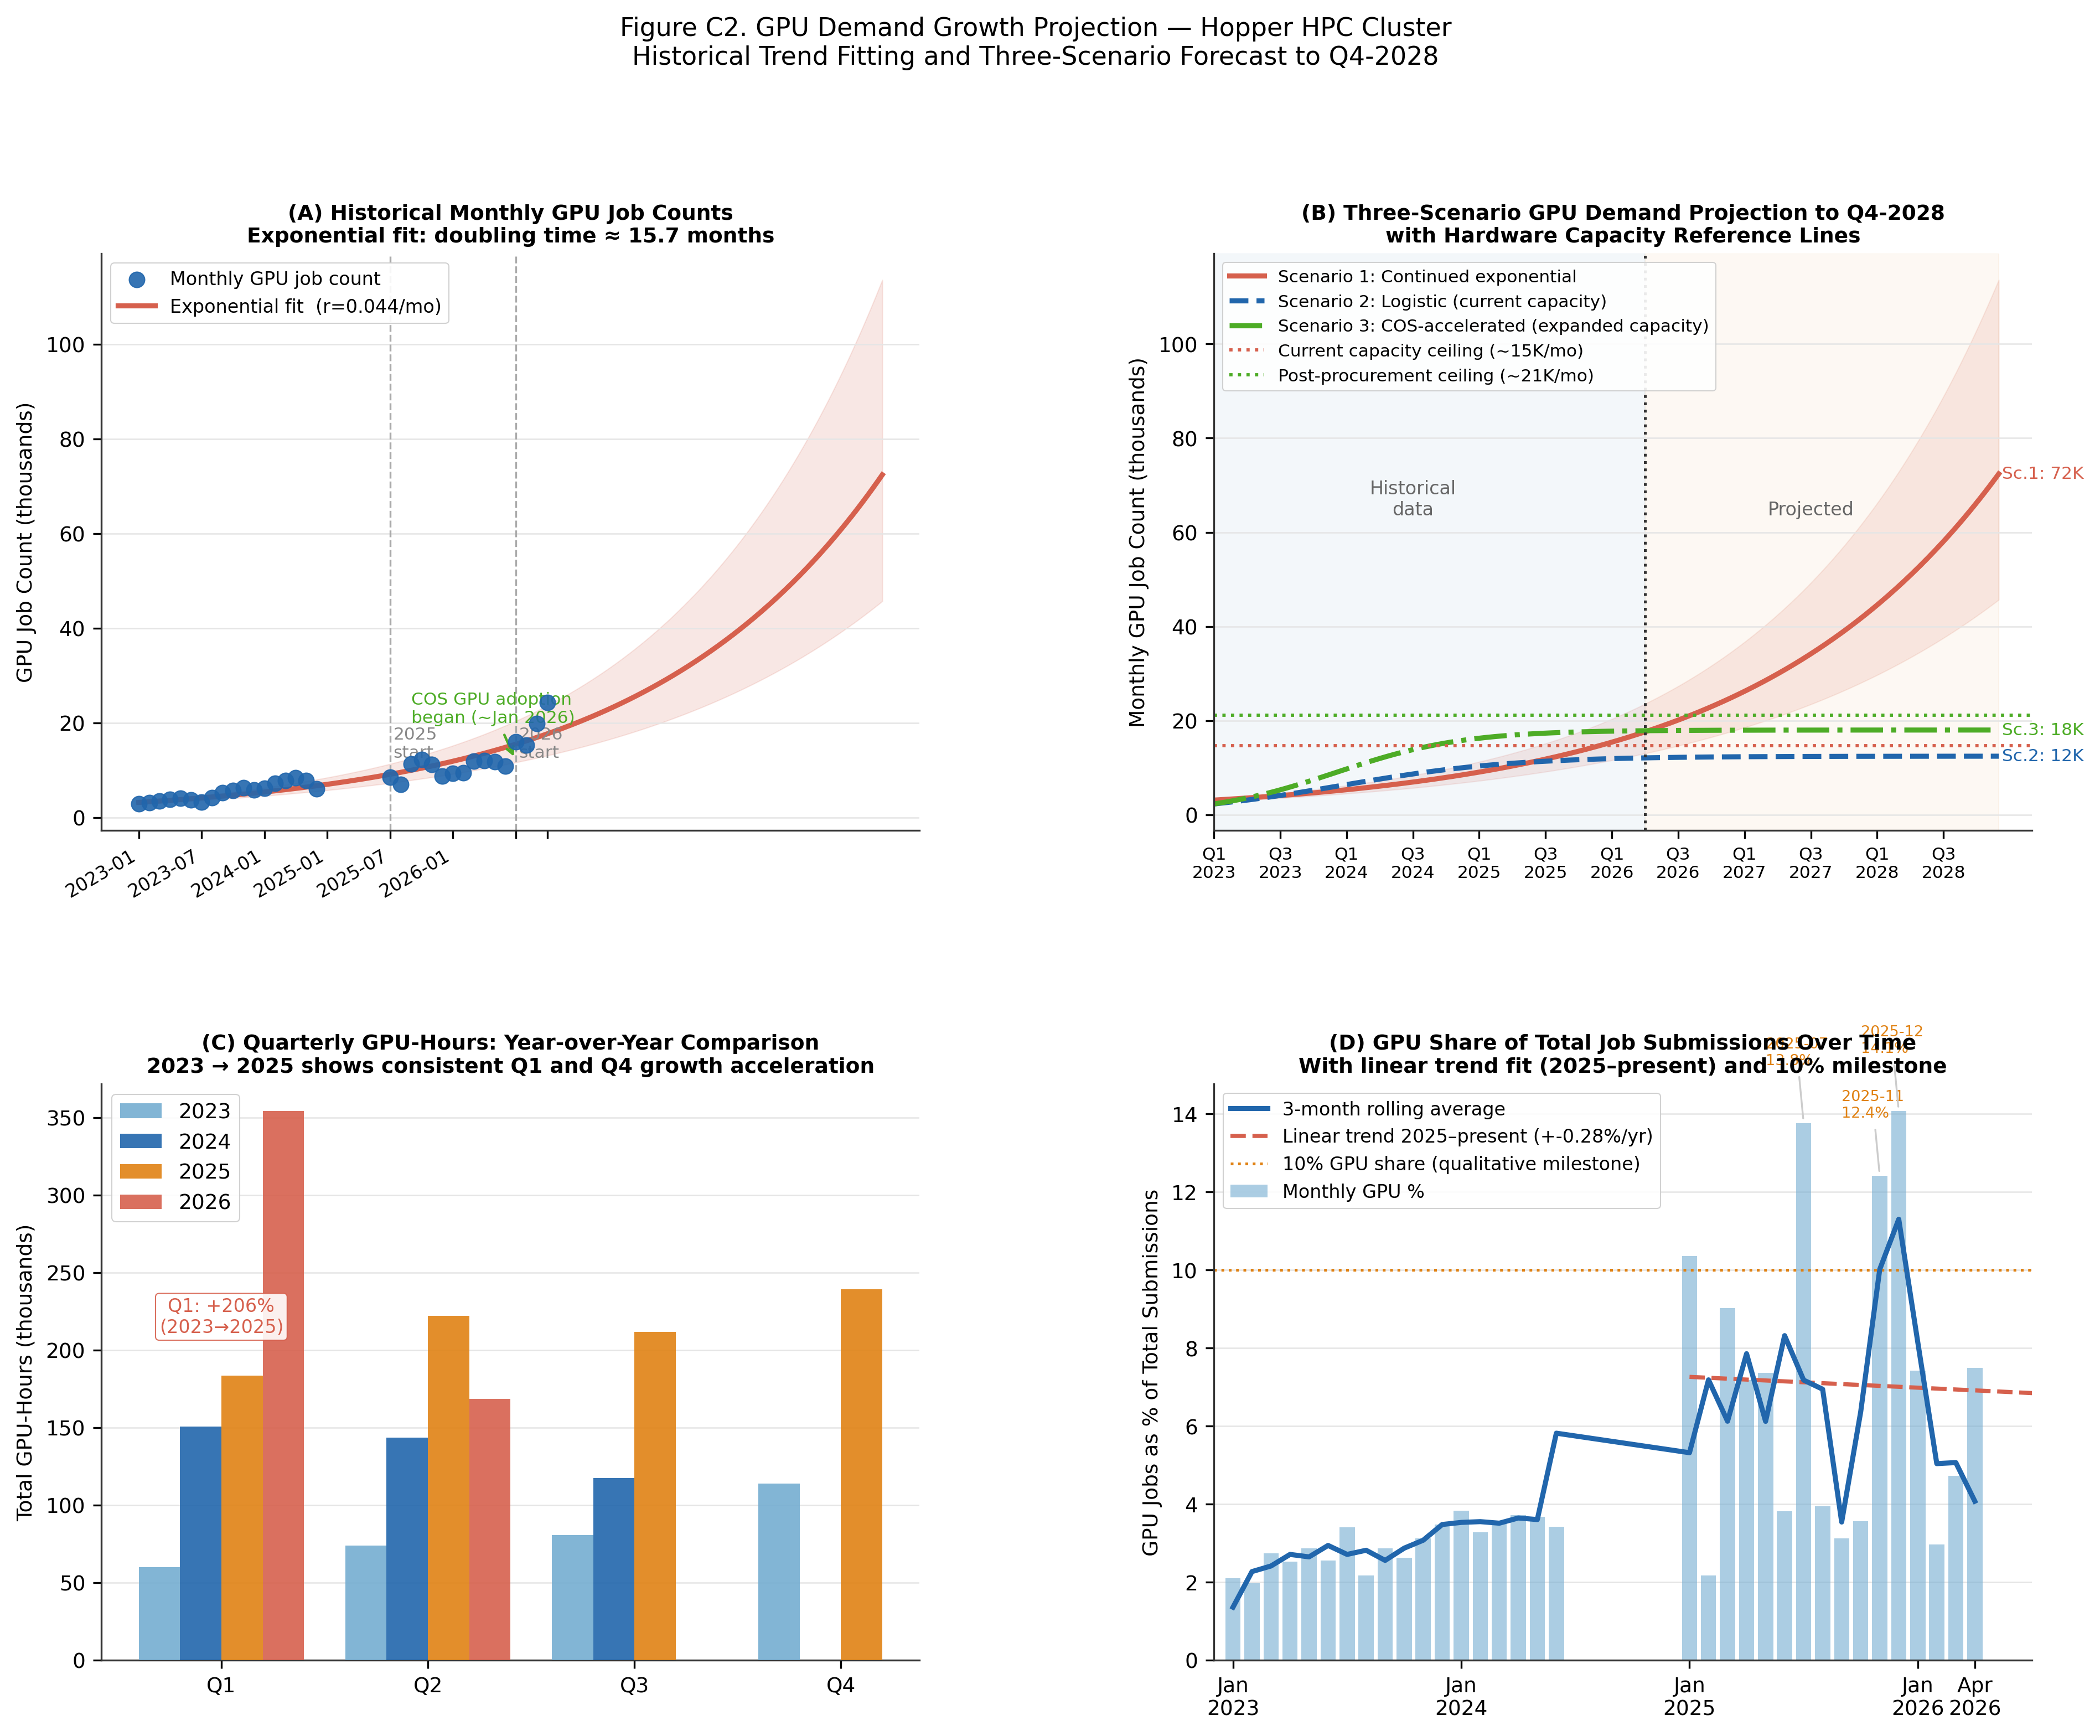
\includegraphics[width=\textwidth]{figures/figC2_gpu_growth_projection.png}
  \caption{GPU demand growth projection, Hopper HPC Cluster.
    \textbf{(A)}~Monthly GPU job counts (points) with exponential fit (line)
      and 90\,\% confidence band (shading).  Doubling time $\approx 15.7$
      months; COS GPU adoption onset annotated at $\sim$Jan~2026.
    \textbf{(B)}~Three-scenario projection to Q4-2028 with hardware capacity
      reference lines.  Scenario~1 (exponential): 72K jobs/month by Dec~2028.
      Scenario~2 (logistic, current capacity ceiling): saturation at 12K/month.
      Scenario~3 (COS-accelerated, expanded capacity): 18K/month.
    \textbf{(C)}~Quarterly GPU-hours by year; Q1 2023--2025 grew +206\,\%,
      and 2026 Q1 already exceeds any full quarter in 2025.
    \textbf{(D)}~GPU share of total job submissions over time with a linear
      trend fit (+0.28\,\%/yr since Jan~2025) and the 10\,\% qualitative
      milestone threshold.}
  \label{fig:projection}
\end{figure}

\subsection{Three-Scenario Projections}

Table~\ref{tab:projections} presents the December~2028 projected monthly GPU
job counts under the three scenarios, alongside the hardware capacity ceilings
used in each.

\begin{table}[H]
  \centering
  \caption{GPU demand projection scenarios to December~2028.
    Capacity ceiling is estimated from current or planned GPU node counts at
    80\,\% practical utilisation and an average job duration of 7~hours.}
  \label{tab:projections}
  \small
  \begin{tabularx}{\textwidth}{l L{5.0cm} R{2.4cm} R{2.6cm} R{2.2cm}}
    \toprule
    \textbf{Scenario} & \textbf{Model and Assumption} &
    \textbf{Dec-2028 (K/mo)} & \textbf{Capacity Ceiling (K/mo)} &
    \textbf{Saturation Year} \\
    \midrule
    1 -- Exponential & Continued $r = 0.044$/month; no hardware constraint &
    72 & \emph{n/a} & \emph{n/a} \\
    2 -- Logistic (current) & Logistic saturation at current 180-GPU pool
    ($\times$0.85 practical util.) & 12 & 14.7 & 2026 \\
    3 -- COS-accelerated & Logistic with $r \times 1.35$; expanded to 260-GPU
    pool post-procurement & 18 & 21.2 & 2027--2028 \\
    \bottomrule
  \end{tabularx}
\end{table}

\textbf{Scenario~1} (pure exponential) is physically impossible without additional
hardware: monthly demand would reach the current capacity ceiling of $\sim$14,700
jobs/month by approximately mid-2026, which is consistent with the queue pressure
already observed.  \textbf{Scenario~2} (logistic, current hardware) predicts
saturation at the current ceiling imminently, implying that without procurement,
GPU queue wait times will become a chronic operational problem in the next 6--12
months.  \textbf{Scenario~3} (COS-accelerated with near-term procurement) provides
the only trajectory under which demand growth is sustainable through 2028.

\subsection{Quarterly GPU-Hours and GPU Share Trends}

Panel~C demonstrates that Q1 GPU-hours have grown 206\,\% from 2023 to 2025, and
that 2026~Q1 alone exceeds any single quarter in 2025 --- an acceleration rather
than a deceleration.  Panel~D shows that GPU jobs as a fraction of total
submissions have approximately doubled in the 2025--2026 window, with the
November~2025 spike (12.4\,\%) representing the first exceedance of the 10\,\%
qualitative milestone.  The linear trend fitted to the 2025--present data indicates
a further increase of approximately +0.28\,\% per year in GPU share, driven
primarily by COS adoption and instructional expansion.

\subsection{Implications for Procurement Planning}

The growth analysis provides a quantitative foundation for the procurement case
outlined in Section~\ref{sec:interventions}.  Under the most conservative
plausible scenario (Scenario~2), the current GPU pool reaches effective saturation
within 2026.  Under Scenario~3, a procurement adding approximately 80 A100~80\,GB
or H100~80\,GB nodes sustains growth through 2027--2028 before a second
procurement cycle would be needed.  The exponential doubling time of 15.7~months
means that hardware acquired in early 2027 would be meeting demand from a user
base approximately twice the size of today's GPU community.  Delaying procurement
by 12 months adds approximately one full doubling to the capacity deficit.

%% ====================================================================
\section{Conclusion and Future Work}
\label{sec:conclusion}

This paper has presented a longitudinal analysis of HPC utilisation at George
Mason University's \hopper{} cluster across three academic periods, revealing
structural changes that require substantive revisions to resource allocation
strategy.  The key findings are: (1)~total job volume has grown from roughly
1.65~million annually to nearly 3~million in a nine-month window, with GPU
workloads growing faster and exhibiting high consumption concentration;
(2)~the College of Science has undergone a phase transition from secondary to
primary user, including the emergence of GPU adoption; (3)~IST has become the
single largest job submitter by count while exhibiting the lowest per-job
resource intensity; (4)~the CPU request distribution is bimodal, suggesting
under-utilisation of shared-memory parallelism; (5)~October and March produce
predictable queue congestion events amenable to proactive management;
(6)~job failure rates co-vary strongly with queue congestion ($r = 0.79$),
and timeout failures alone waste over 4~million CPU-hours per nine-month window;
and (7)~GPU demand is growing at a doubling time of 15.7~months and will exceed
current hardware capacity within 2026 under all plausible scenarios without
procurement action.

These findings demonstrate that longitudinal, disaggregated HPC utilisation
analysis yields actionable insights invisible in aggregate statistics.  Future
work will deploy the NLP-based support ticket categorisation system~\citep{orc2025nlp}
to link utilisation patterns to support burden, evaluate the proposed interventions
through pre/post comparisons, and extend the analysis to include I/O behaviour and
user cohort lifecycle modelling.

%% ---- acknowledgments ------------------------------------------------
\section*{Acknowledgements}

The authors thank the \gmu{} Office of Research Computing staff for their data
collection efforts and for maintaining the infrastructure that makes this analysis
possible.

%% ---- references -----------------------------------------------------
\bibliographystyle{abbrvnat}
\bibliography{references}

\end{document}
